% !TEX TS-program = XeLaTeX
% Commands for running this example:
% 	 xelatex vahid-seminar
% 	 xelatex vahid-seminar
% End of Commands


%%%  نمونه یک سمینار کارشناسی ارشد، دانشگاه تبریز،  وحید دامن ‌افشان،     vdamanafshan@yahoo.com 


% توجه داشته باشید برای دیدن خروجی کامل شامل نمایه و فهرست مطالب در ویرایشگر Texmaker، ابتدا دو بار 
% کلید F1 و بعد کلید F12 و دوباره کلید F1 و در آخر کلید F7 را فشار دهید.
% توضیحات مربوط به هر بسته یا دستور را می‌توانید در خط بالای آن ببینید.

\documentclass[12pt,a4paper]{article}
%در ورژن جدید زی‌پرشین برای تایپ متن‌های ریاضی، این سه بسته، حتماً باید فراخوانی شود
\usepackage{amsthm,amssymb,amsmath}
%بسته‌ای برای تنطیم حاشیه‌های بالا، پایین، چپ و راست صفحه
%\usepackage[top=50mm, bottom=50mm, left=50mm, right=50mm]{geometry}

\usepackage{graphicx}
% بسته‌ و دستوراتی برای ایجاد لینک‌های رنگی با امکان جهش 
\usepackage[pagebackref=true,colorlinks,linkcolor=blue,citecolor=magenta]{hyperref}
% چنانچه قصد پرینت گرفتن نوشته خود را دارید، خط بالا را غیرفعال و  از دستور زیر استفاده کنید چون در صورت استفاده از دستور زیر‌‌، 
% لینک‌ها به رنگ سیاه ظاهر خواهند شد و برای پرینت گرفتن، مناسب‌تر است
%\usepackage[pagebackref=false]{hyperref}
% بسته‌ای برای ظاهر شدن «مراجع» و« نمایه» در فهرست مطالب
\usepackage{tocbibind}
% دستورات مربوط به ایجاد نمایه
\usepackage{makeidx}
\makeindex
%%%%%%%%%%%%%%%%%%%%%%%%%%
% فراخوانی بسته زی‌پرشین و دستورات مربوط به نوع فونت‌ها
\usepackage{xepersian}
\settextfont[Scale=1.1]{XB Niloofar}
%\setlatintextfont[Scale=2]{Linux Libertine}
%\setlatintextfont[Scale=1]{Times New Roman}
% از revision 118 زی‌پرشین به بعد، وارد کردن دستور زیر لازم نیست. توجه داشته باشید که در صورت  غیرفعال کردن این دستور،
% از فونت پیش‌فرض لاتک برای کلمات انگلیسی استفاده خواهد شد.
%\setlatintextfont[ExternalLocation,BoldFont={lmroman10-bold},BoldItalicFont={lmroman10-bolditalic},ItalicFont={lmroman10-italic}]{lmroman10-regular}
% چنانچه می‌خواهید اعداد در فرمول‌ها، فارسی باشد، خط زیر را نیز فعال کنید
%\setdigitfont[Scale=1.1]{XB Zar}
%%%%%%%%%%%%%%%%%%%%%%%%%%
% تعریف قلم‌های فارسی و انگلیسی برای استفاده در بعضی از قسمت‌های متن
\defpersianfont\titr[Scale=1]{XB Titre}
\defpersianfont\nastaliq[Scale=1.5]{IranNastaliq}
%\defpersianfont\traffic[Scale=1]{B traffic}
% چنانچه فونت B Traffic را ندارید، دستور بالا را غیرفعال کرده و دستور زیر را فعال کنید
\defpersianfont\traffic[Scale=1]{XB Niloofar}
%%%%%%%%%%%%%%%%%%%%%%%%%%
%تعریف و نحوه ظاهر شدن عنوان قضیه‌ها، تعریف‌ها، مثال‌ها و ...
\theoremstyle{definition}
\newtheorem{definition}{تعریف}[section]
\theoremstyle{theorem}
\newtheorem{theorem}[definition]{قضیه}
\newtheorem{lemma}[definition]{لم}
\newtheorem{proposition}[definition]{گزاره}
\newtheorem{corollary}[definition]{نتیجه}
\newtheorem{remark}[definition]{ملاحظه}
\theoremstyle{definition}
\newtheorem{example}[definition]{مثال}

%%%%%%%%%%%%%%%%%%%%%%%%%%
% تعریف دستورات جدید برای خلاصه نویسی و راحتی کار در هنگام تایپ فرمول‌های ریاضی
\newcommand{\bR}{\mathbb{R}}
\newcommand{\cB}{\mathcal{B}}
\newcommand{\cO}{\mathcal{O}}
\newcommand{\cG}{\mathcal{G}}
\newcommand{\rM}{\mathrm{M}}
\newcommand{\rC}{\mathrm{C}}
\newcommand{\rV}{\mathrm{V}}
\newcommand{\ls}{\mathrm{LSC}_{+}(X)}
\newcommand{\ce}{\mathrm{C}^{*}(X)}
%%%%%%%%%%%%%%%%%%%%%%%%%%
% تغییر نام کلمه «اثبات» به «برهان»
\renewcommand\proofname{\textbf{برهان}}
%%%%%%%%%%%%%%%%%%%%%%%%%%
\begin{document}
% دستوری برای زدن شماره صفحه‌ها به صورت الف، ب، ج و ... (معمولاً در در هر نوشته‌ای، شماره صفحات تا شروع فصل 
% اول آن متن را به صورت الف، ب، ج و ... وارد می‌کنند)
\pagenumbering{harfi}
% دستوری جهت ظاهر نشدن شماره صفحه (فقط در صفحه جاری)
\thispagestyle{empty}
% دستوری برای کم کردن فاصله بین لوگو و لبه بالایی صفحه خروجی
\vspace*{-19mm}
% نحوه درج کردن لوگوی دانشگاه
\centerline{
\includegraphics[height=4cm]{logo2.jpg}}

\begin{center}
% دستوری برای کم کردن فاصله بین لوگو و خط پایین آن
\vspace{-3mm}
دانشکده علوم ریاضی
% دستوری برای تعیین فاصله بین دو خط
\\[.2cm]

گروه ریاضی محض
\\[1.7cm]
{\Large 
\textbf{سمینار کارشناسی ارشد با عنوان}
}
\\[.8cm]
{\titr
\begin{Huge}
دامنه توانی احتمالی برای فضاهای فشرده 
\\[.4cm]
پایدار با استفاده از فضاهای مرتب فشرده
\end{Huge}}
\\[1.3cm]
{\Large {\traffic 
استاد راهنما
}
\\[.7cm]
{\Large \nastaliq دکتر - - - - }
\\[.9cm]
{\Large\traffic  پژوهشگر
}}
\\[.7cm]
{\Large \nastaliq وحید دامن‌افشان}
\\[1.8cm]
 تابستان ۱۳۸۸
\end{center}

% دستوری برای رفتن به صفحه جدید
\newpage
% دستوری برای تعیین فاصله بین خطوط (نه دو خط) و تا وقتی که مقدار آن تغییر نکند، فاصله بین خطوط، همین مقدار است
\baselineskip=1cm
% دستوری برای ظاهر شدن فهرست مطالب
\tableofcontents
\newpage
\baselineskip=.750cm
% دستوری برای اختصاص دادن یک عدد به شماره صفحه جاری
%\setcounter{page}{3}
% دستوری برای زدن شماره صفحه‌ها به صورت ۱، ۲، ۳ و ...
\pagenumbering{arabic}

\section*{چکیده}
این سمینار که بر اساس مرجع 
\cite{main}
تنظیم شده است، به بحث در مورد فضاهای فشرده پایدار و فضاهای مرتب فشرده می‌پردازد.
فضاهای فشرده پایدار 
$ X_{s} $
در واقع از ضعیف کردن توپولوژی فضاهای مرتب فشرده 
$ X $
به مجموعه‌های بالایی باز ناشی می‌شود. در این سمینار به بررسی دامنه توانی احتمالی یک فضای فشرده پایدار 
$ X_{s} $
با استفاده از فضای مرتب فشرده 
$ X $
و ابزارهای کلاسیک نظریه اندازه و آنالیز تابعی می‌پردازیم. این کار به ما اجازه می‌دهد که یک روش زیبا، جمع ‌و جور و مشهور و همچنین نتایج جدیدی که در قضیه
\ref{5.4}
 خلاصه شده است را نتیجه بگیریم.\\
\textit{واژه های کلیدی:}
دامنه‌های معنایی،  دامنه توانی احتمالی،  فضاهای فشرده پایدار.
\section{مقدمه}
درمعنی شناسی نمادین\LTRfootnote{Denotational semantics}،  ارزیابی‌ها و دامنه‌توانی احتمالی توسط جونز\LTRfootnote {Jones}و پلاتکین\LTRfootnote {Plotkin }\cite{Jones}
به عنوان جایگزینی برای احتمالات و فضای اندازه‌های احتمال، به منظور مدل بندی پدیده‌‌‌‌‌‌‌های احتمالی در برنامه‌ریزی معرفی شده است. اخیراً به دامنه توانی احتمالی توجه بیشتری شده است. بیشتر پیش‌زمینه‌ها در بحث دامنه توانی احتمالی بجز چند خاصیت اصلی که در
\cite{G. Gierz}
 آمده است همگی در پایان‌نامه‌هایی است که دسترسی به آنها به آسانی امکان‌پذیر نیست.


مبحث معنی ‌شناسی نمادین، بر پایه نظریه فضاهای متریک یا نظریه دامنه از دیدگاه 
\linebreak
 دی. اس. اسکات\LTRfootnote {D.S. Scott}
پایه‌گذاری شده است.  به منظور بحث درباره اندازه‌ها و احتمالات برای معنی شناسی، باید مفاهیم کلاسیکی اندازه،  احتمال و انتگرال را با دامنه‌ها سازگار کنیم.  یک دامنه، 
\index{دامنه}
یک مجموعه مرتب  جزیی کامل جهت‌دار پیوسته است (\cite{G. Gierz}
 را ببینید). هر دامنه،  یک توپولوژی ذاتی، توپولوژی اسکات، که
$ T_{0} $
بوده و هاسدورف نیست را حمل می‌کند. ارزیابی‌ها که طبق تعریف، نوعی از اندازه را به هر مجموعه اسکات-باز مرتبط می‌کنند، جای اندازه‌ها را می‌گیرند. ارزیابی‌ها روی یک دامنه از یک دامنه در خودش، دامنه توانی احتمالی توسعه‌یافته نامیده می‌شود.
 
 البته مایلیم که ارزیابی‌ها را به اندازه های کلاسیک، و دامنه توانی احتمالی توسعه یافته را به فضای همه اندازه‌ها بازگو کنیم.
 
 نظریه اندازه توپولوژیکی،  
 \index{نظریه اندازه توپولوژیکی}
 تقریباً و منحصراً به بحث در مورد فضاهای هاسدورف، بخصوص به فضاهای موضعاً فشرده و فضاهای متریک تام پرداخته است. بنابراین،  طبیعی است که دامنه‌هایمان را به دامنه‌هایی که برای توپولوژی لاوسون\LTRfootnote{Lawson}، هاسدورف فشرده هستند محدود کنیم که این توپولوژی لاوسون یک توپولوژی ذاتی روی دامنه‌هایی است که توپولوژی اسکات را تظریف می‌کنند. این محدودیت زیاد سنگین نیست به طوری که همه دامنه‌های مشمول در یک رسته بسته دکارتی از دامنه‌ها، فشرده لاوسون هستند(\cite{Jung}  
  را ببینید). دامنه‌هایی که لاوسون فشرده هستند، فشرده پایدار نیز نامیده می‌شوند. این کار ما را به تفکر بیشتر درباره فضاهای فشرده پایدار که اخیراً در مبحث معنی‌شناسی نیز خیلی مفید هستند،  سوق می‌دهد(\cite{Kegelmann}  
را ببینید). فضاهای فشرده پایدار
 $ \left( X,\mathcal{G}\right)  $
 از دیدگاه
 %\linebreak
  ناخبین\LTRfootnote{Nachbin}\cite{Nachbin}
 دقیقاً فضاهایی هستند که از فضاهای مرتب فشرده 
 $\left( X,\mathcal{G},\leq\right)$، با ضعیف کردن توپولوژی آن به گردایه 
 $\mathcal{G}  $
 از همه مجموعه‌های بالایی باز، ناشی می‌شوند.
 
 برای اینکه بحث ما برای خوانندگانی که با نظریه دامنه آشنایی ندارند، ساده و قابل فهم باشد ما بیشتر روی  فضاهای مرتب فشرده کار می‌کنیم. ما از آنالیز تابعی کلاسیک از یک طرف برای نتیجه‌گیری ارتباط نزدیک بین ارزیابی‌ها روی فضای فشرده پایدار 
 $ \left( X,\mathcal{G}\right)  $
 و خصوصیات دامنه توانی احتمالی روی چنین فضایی،  و از طرف دیگر اندازه‌های بورل منتظم و مجموعه محدب فشرده‌ای از اندازه‌های احتمال روی 
 $ \left( X,\mathcal{O}\right)  $
 در ضعیف*-توپولوژی استفاده می‌کنیم.  همه نتایج ما بخصوص برای دامنه‌هایی که فشرده لاوسون هستند بکار می‌روند.
 

\section{تعاریف و مفاهیم اولیه}
تعاریف و قضیه‌های بکار رفته در این قسمت، بجز مواردی که به روشنی ذکر شده است، از مرجع 
\cite{abramsky2}
گرفته شده‌اند.
\begin{definition}\label{d1} 
مجموعه 
$ P $
همراه با رابطه دوتایی 
$ \leq $، یک مجموعه جزئاً مرتب یا
\index{مجموعه!جزئاً مرتب}
\lr{poset}،  نامیده می‌شود هرگاه شرایط زیر برای هر 
$ x,y,z \in P$\index{$ poset $}
برقرار باشد:
\begin{LTR}
\begin{description}
\item{(1}   
$ x\leq x  $  \ \ \  \rl{(بازتابی)} 
\item{(2}
$ x\leq y \bigwedge y\leq z \Longrightarrow x\leq z $ \ \ \  \rl{(تعدی)}
\item{(3}
$ x\leq y \bigwedge y \leq x \Longrightarrow x=y  $\ \ \ \rl{(پادتقارنی)}
\end{description}
\end{LTR}
\end{definition}
\begin{definition}
اگر شرط پادتقارنی را از تعریف
\ref{d1}
برداریم، چیزی که به دست می‌آید، یک \textbf{پیش‌ترتیب}\LTRfootnote{Preorder}
است.
\index{بیی@پیش‌ترتیب}
\end{definition}

\begin{definition}
فرض کنید
$ (P,\leq) $
یک مجموعه جزئاً مرتب باشد.
\begin{enumerate}
\item 
زیرمجموعه 
$ A $
از 
$ P $
یک \textbf{مجموعه بالایی} 
است 
\index{مجموعه!بالایی}
اگر 
$ x\in A $
برای هر
$ y\geq x $، 
$ y\in A $
را ایجاب کند.  مجموعه همه عناصر بالای عضوی از 
$ A $
را با
$ \uparrow A $\index{$ \uparrow A $}
نشان می‌دهیم.   هرگاه بیم اشتباه نرود،  
$ \uparrow \left\lbrace x\right\rbrace  $\index{$ \uparrow \left\lbrace x\right\rbrace  $}
را به صورت 
$ \uparrow x $\index{$ \uparrow x $}
نشان می‌دهیم.  \textbf{مجموعه پایینی} و 
$ \downarrow A $، بطور مشابه تعریف می‌شوند.
\item
عنصر
$ x\in P $
\textbf{کران بالا}
 \index{قییی@کران بالا}
 برای زیرمجموعه 
$ A\subseteq P $
نامیده می‌شود هرگاه 
$ x $، بالای هر عنصری از 
$ A $
باشد. این حالت را معمولاً با 
$ A\leq x $\index{$ A\leq x $}
نشان می‌دهیم.  مجموعه همه کران‌های بالای 
$ A $
را با 
$ \mathrm{ub}(A) $\index{$ \mathrm{ub}(A) $}
نشان می‌دهیم.
\item
عنصر 
$ x\in P $
\textbf{ماکسیمال}
\index{عنصر!ماکسیمال}
است اگر هیچ عنصر دیگری از 
$ P $،  بالای آن نباشد؛ به عبارت دیگر
$ \uparrow x \bigcap P=\left\lbrace x\right\rbrace  $%
. عنصر مینیمال 
\index{عنصر!مینیمال} 
نیز بطور مشابه تعریف می‌شود.
\item
اگر همه عناصر
$ P $، پایین عنصری مانند
$ x\in P $
باشند آنگاه 
$ x $
\textbf{بزرگ‌ترین عنصر}
\index{بزرگ‌ترین عنصر}
 نامیده می‌شود.   تعریف مشابه، 
\textbf{کوچک‌ترین عنصر}
\index{قییی@کوچک‌ترین عنصر}
 است که 
 \textbf{عنصر زیر}\LTRfootnote{Bottom element}
 \index{عنصر!زیر}
 نیز نامیده می‌شود.
\item
اگر برای زیرمجموعه 
$ A\subseteq P $، مجموعه کران‌های بالای $ A $، یک کوچک‌ترین عنصر 
$ x $
را داشته باشند،  آنگاه
$ x $
\textbf{سوپریمم}
\index{سوپریمم}
یا
\textbf{مفصل}\LTRfootnote{Join}
\index{مفصل}
$ A $ نامیده می‌شود و آن را به صورت 
$ x=\bigsqcup A $\index{$ x=\bigsqcup A $}
نشان می‌دهیم.
\end{enumerate}
\end{definition}



\begin{definition}
 فرض کنید 
 $ P $
 و
 $ Q $
 دو مجموعه جزئاً مرتب باشند.  تابع 
 $ f:P\rightarrow  Q$
 \textbf{یکنوا}
 \index{تابع!یکنوا}
 نامیده می‌شود هرگاه برای هر 
 $ x,y\in P $
 با شرط 
 $ x\leq y $، در 
 $ Q $
 نیز داشته باشیم
 $ .f(x)\leq f(y) $
 \end{definition}
\begin{definition}[\cite{lawson 2}]
فرض کنید 
$ \mathcal{A} $،   جبر زیرمجموعه‌های مجموعه ناتهی $  X$
 باشد.  یک 
 %\linebreak
\textbf{$\mathcal{A} $-افراز}\LTRfootnote{$\mathcal{A}-partition$}
\index{$ \mathcal{A} $-افراز}
مجموعه $ X $، افرازی توسط زیرمجموعه‌هایی است که همه آنها متعلق به  
$ \mathcal{A} $
 هستند.
\end{definition}
\begin{definition}[\cite{lawson 2}]
فرض کنید $ X $ یک فضای توپولوژیک باشد.  
تابع کراندار $ f:X\rightarrow \bR $، \lr{S}-انتگرال‌پذیر 
\index{تابع!\lr{s}-انتگرال‌پذیر}
است (نسبت به جبر $ \mathcal{A} $ و اندازه کراندار نامنفی جمع‌پذیر متناهی $  \mu$)،  هرگاه انتگرال بالایی و پایینی $ f $،  متناظر با $ \mu $ و $  \mathcal{A} $، با هم مساوی باشد که این انتگرال بالایی و پایینی به ترتیب  بصورت 
$$\overline{\int}fd\mu=\inf_{\mathcal{P}}S^{u}(f,\mu,\mathcal{P})$$
و
$$\underline{\int}fd\mu=\sup_{\mathcal{P}}S^{l}(f,\mu,\mathcal{P})$$
تعریف می‌شوند که در آن 
$ \mathcal{P} $
، یک $\mathcal{A} $-افراز متناهی $ X $  است و 
$$S^{u}(f,\mu,\mathcal{P})=\sum_{P\in\mathcal{P}} \sup f(P)\mu(P)$$\index{$S^{u}(f,\mu,\mathcal{P})$}
و
$$S^{l}(f,\mu,\mathcal{P})=\sum_{P\in\mathcal{P}}\inf f(P)\mu(P).$$\index{$ S^{l}(f,\mu,\mathcal{P}) $}
از آنجایی که $  f$ و $  \mu$ کراندارند لذا 
$S^{u}(f,\mu,\mathcal{P})$
و
$S^{l}(f,\mu,\mathcal{P})$
خوش‌تعریف‌اند و آنها را به ترتیب مجموع بالایی داربوکس
\LTRfootnote{Darboux sum}
\index{مجموع داربوکس}
 و مجموع پایینی داربوکس $ f $ متناظر با $ \mu $ و
$\mathcal{A} $-افراز 
متناهی $ \mathcal{P} $ می‌نامند.\\
اگر $  f$، \lr{S}-انتگرال‌پذیر             باشد، انتگرال $  f$ را ریمان-اشتیلیس
 \index{انتگرال!ریمان-اشتیلیس}
 می‌نامند و با 
$ S\int fd\mu $ 
نشان می‌دهند.
\end{definition}
\begin{definition}[\cite{Jung and Tix}]
فرض کنید
$ (X,\tau) $
یک فضای توپولوژیکی باشد.   یک
\textbf{ارزیابی}\LTRfootnote{Valuation}%
\index{ارزیابی}%
روی 
$ X $
  تابعی مانند 
$ \mu:\tau\rightarrow [0,1]\subseteq \bR $
با خواص زیر است
\begin{itemize}
\item
$ \mu $
اکید است:
$ \mu(\emptyset)=0 $
\item
$ \mu $
مدولار 
\index{مدولار}
است:
$ \mu(U)+\mu(V)=\mu(U\cup V)+\mu(U\cap V) $
\item
$ \mu $
 یکنوای صعودی است:
$ .U\subseteq V \ \ \rightarrow \mu(U)\subseteq \mu(V) $
\end{itemize}
\end{definition}

\begin{definition}[\cite{lawson 2}]
فرض کنید $ \mu $ یک ارزیابی و $  f$ تابعی از $ X $ به 
$\overline{\bR}  $
باشد.  \textbf{انتگرال افقی}\LTRfootnote{Horizontal integral} 
\index{انتگرال!افقی}
تابع $ f $ بطور مستقیم  از ارزیابی $ \mu $ بصورت 
$$\int_{X}fd\mu=\int_{0}^{\infty}f^{\mu}(r)dr$$
تعریف می‌شود که در آن 
$$f^{\mu}(r)=\mu\left( f^{-1}\left(]r,\infty]\right) \right). $$
از آنجایی که $  f^{\mu}$ نزولی یکنوا است لذا می‌بینیم که انتگرال ریمان ناسره $ \int_{0}^{\infty}f^{\mu}(r)dr $ وجود دارد و یا همگرا به مقداری متناهی و یا واگرا به $ \infty $ است.
\end{definition}
\begin{proposition}[\cite{lawson 2}]\label{p1} 

برای یک تابع کراندار اندازه‌پذیر   
$f:X\rightarrow \overline{\bR}$، \lr{S}-انتگرال و انتگرال افقی، هر دو موجود و با هم برابر است.
\end{proposition}
\begin{definition}
فرض کنید
$ P $
یک مجموعه جزئاً مرتب باشد.   زیرمجموعه
$ A $
از
\mbox{$ P $\textbf{جهت‌دار}\LTRfootnote{Directed}}
\index{مجموعه!جهت‌دار}
است هرگاه ناتهی بوده و هر زوج از عناصر
$ A $، یک کران بالا در 
$ A $
داشته باشند.   اگر  مجموعه جهت‌دار 
$ A $، یک سوپریمم داشته باشد آن را با 
$ \bigsqcup^{\uparrow}A $\index{$ \bigsqcup^{\uparrow}A $}
نشان می‌دهیم.
\end{definition}
\begin{definition}
یک 
\textbf{تور}\LTRfootnote{Net}
\index{تور}
در فضای توپولوژیکی $ (X,\tau) $،  تابعی مانند 
\begin{align}
f:I\rightarrow X\nonumber \\
f(\alpha)=x_{\alpha}\nonumber
\end{align}
است که در آن $ I $،  یک مجموعه جهت‌دار است ومعمولاً با
 $ \left\lbrace x_{\alpha}\right\rbrace  $
  نشان می‌دهیم.  اگر تابع $ f $، یکنوا باشد آن را 
یک \textbf{تور یکنوا}\LTRfootnote{Monotone net} 
\index{تور!یکنوا}
می‌نامیم. مجموعه 
$ I $،   
\textbf{مجموعه اندیس‌گذار}
\index{مجموعه!اندیس‌گذار}
تور نامیده می‌شود.
\end{definition}
\begin{definition}
یک \textbf{مخروط}\LTRfootnote{Cone}
\index{مخروط}
  عبارت است از یک مجموعه مانند $  \mathcal{P}$ همراه با یک عمل جمع 
$ (a,b)\mapsto a+b $
 و یک ضرب عددی 
  $(\alpha , a)\mapsto \alpha a  $
 که در آن
  $ \alpha\geq 0 $
   و  کلیه خواص یک فضای برداری را داشته باشد.
\end{definition}

\begin{definition}
مجموعه جزئاً مرتب 
$ D $
که هر زیرمجموعه جهت‌دار آن، یک سوپریمم دارد،  مجموعه جزئاً مرتب کامل جهت‌دار و یا به اختصار، یک 
\textbf{\lr{dcpo}}
\index{$ poset $}
نامیده می‌شود.
\end{definition}
\begin{definition}[\cite{lawson 2}]
یک \textbf{\lr{dcpo}-مخروط}\LTRfootnote{Dcpo-cone}،  
\index{\lr{dcpo}-مخروط}
عبارت است از یک \lr{dcpo}ی $ D $ مجهز به یک عنصر متمایز $ 0\in D $ و یک جمع 
$ +:D\times D\rightarrow D $
و یک ضرب اسکالر 
$ \cdot:\bR^{+}\times D\rightarrow D $%
،  بطوری‌که کلیه خواص یک فضای برداری، بجز خاصیت معکوس جمعی برقرار باشد (در این حالت باید فرض کنیم که برای هر 
$ a\in D $،  $ 0\cdot a=0 $%
).
\end{definition}
\begin{definition}
فرض کنید مجموعه‌های
$ D $
و
$ E $
دو 
$ \mathrm{dcpo} $
باشند.   تابع 
$ f:D\rightarrow E $، 
\linebreak 
 \textbf{(اسکات-) پیوسته} 
 \index{تابع!(اسکات-)پیوسته}
 نامیده می‌شود هرگاه یکنوا بوده و برای هر زیرمجموعه جهت‌دار 
$ A $
از
$ D $
داشته باشیم
$ f(\bigsqcup^{\uparrow}A) =\bigsqcup^{\uparrow}f(A)$.  مجموعه همه توابع پیوسته یکنوای نقطه‌وار    از
$ D $
به 
$ E $
را با
$ [D\longrightarrow E] $\index{$ [D\longrightarrow E] $}
نشان می‌دهیم.   توابع بین 
$ \mathrm{dcpo} $های جهت‌دار که عنصر زیر را حفظ می‌کنند، 
\textbf{اکید}
\index{تابع!اکید}
نامیده می‌شوند.
\end{definition}
\begin{definition}
فرض کنید 
$ D $
یک 
$ \mathrm{dcpo} $
باشد. زیر مجموعه 
$ A $،   
\textbf{(اسکات-)بسته}
 \index{مجموعه!اسکات-بسته}
 است هرگاه یک مجموعه پایینی بوده و تحت سوپریمم زیر مجموعه‌های جهت‌دار،   بسته باشد. 
\end{definition}
 \begin{definition}
فرض کنید 
$ D $
یک 
$ \mathrm{dcpo} $
باشد. 
 \textbf{اسکات-توپولوژی}\LTRfootnote{Scott-topology}
$ \sigma_{D} $
 \index{توپولوژی!اسکات}
 روی $ D $ به صورت زیر تعریف می شود:
 \\
 مجموعه 
 $  O\subseteq D$،  
\textbf{(اسکات-)باز}
\index{مجموعه!اسکات-باز}
است هرگاه یک مجموعه بالایی بوده و برای هر مجموعه جهت‌دار $ A\subseteq D $،  رابطه 
$ \bigsqcup^{\uparrow}A\in O $،  وجود یک $  a\in A\cap O$   را ایجاب کند.

\end{definition}
\begin{definition}
\textbf{توپولوژی لاوسون}\LTRfootnote{Lawson topology}
\index{توپولوژی!لاوسون}
روی یک 
$ \mathrm{dcpo} $ی
$ D $،  کوچکترین توپولوژی شامل همه مجموعه‌های اسکات-باز و همه مجموعه‌های به فرم 
$ D\setminus \uparrow x $\index{$ D\setminus \uparrow x $}
است.
\end{definition}

\begin{definition}[\cite{Nachbin}]
 فضای توپولوژی 
$ X $،   
\textbf{نرمال}
 \index{فضای!نرمال}
 است هرگاه برای هر دو مجموعه بسته و مجزای 
$ E_{1} $
و
$ E_{2} $
در
$ X $،  مجموعه‌های باز 
$ A_{1} $
و
$ A_{2} $
وجود داشته باشند،   بطوری که مجزا بوده و
$ E_{1}\subseteq A_{1} $
و
$ E_{2}\subseteq A_{2} $
باشد.
\end{definition}
\begin{theorem}[جداسازی اوریسون  \cite{Nachbin}، قضیه ۱]\label{or}
\index{قضیه!جداسازی اوریسون}
فضای توپولوژیک $ X $،  نرمال است اگر و تنها اگر برای هر دو  زیرمجموعه بسته مجزای 
$ E_{1},E_{2}\subset X $،   تابع حقیقی و پیوسته  
$ 0\leq f \leq 1 $
روی 
$ X $
چنان باشد که اگر 
$ x\in E_{1} $
آنگاه 
$ f(x)=0 $
و اگر 
$ x\in E_{2} $
آنگاه
$.f(x)=1 $

\end{theorem}
\begin{example}[\cite{Nachbin}]

هر فضای هاسدورف فشرده و هر فضای متریک،  نرمال است.

\end{example}

\begin{definition}[\cite{Nachbin}]
فرض کنید 
$ E $
یک مجموعه پیش‌مرتب باشد.  زیرمجموعه 
$ E_{1}\subseteq E $
\mbox{\textbf{کاهشی}\LTRfootnote{Decreasing}}
\index{مجموعه!کاهشی}
 نامیده می‌شود هرگاه 
$ a\leq b $
و
$ b\in E_{1} $، رابطه 
$ a\in E_{1} $
را ایجاب کند.  مجموعه افزایشی،  
\index{مجموعه!افزایشی}
بطور مشابه تعریف می‌شود.
\end{definition}

\begin{definition}[\cite{Nachbin}]\label{nor}
یک فضای برداری 
$ X $
مجهز  به یک پیش‌ترتیب، 
\textbf{بطور نرمال \linebreak پیش‌مرتب}
 \index{فضای!بطور نرمال پیش‌مرتب}
 نامیده می‌شود هرگاه برای هر دو زیرمجموعه بسته مجزای 
$ E_{1} $
و
$ E_{2} $
از 
$ X $
که 
$ E_{1} $
کاهشی و
$ E_{2} $
افزایشی است، دو زیرمجموعه باز و مجزای 
$ A_{1} $
و
$ A_{2} $
وجود داشته باشد،   بطوری که 
$ A_{1} $
شامل 
$ E_{1} $
و کاهشی و
$ A_{2} $
شامل 
$ E_{2} $
و افزایشی باشد.
\end{definition}
\begin{definition}[\cite{Nachbin}]
فضای برداری 
$ X $
\textbf{بطور نرمال مرتب}
 \index{فضای!بطور نرمال ‌مرتب}
 است هرگاه علاوه بر شرایط تعریف
\ref{nor}، پیش‌ترتیب آن، یک ترتیب باشد.
\end{definition}

\begin{definition}[\cite{Nachbin}]

\textbf{گراف}\LTRfootnote{Graph}
 \index{قیییگراف@گراف}
 یک پیش‌ترتیب روی مجموعه 
$ E $
برابر با مجموعه 
\begin{flushleft}
$ G_{E}=\left\lbrace (x,y)\in E  \times E : x\leq y\right\rbrace $
\end{flushleft}
\index{$G_{E}  $}
است.
\end{definition}
\begin{definition}[\cite{Nachbin}]
یک ترتیب روی فضای توپولوژیکی 
$ X $، \textbf{بسته}
\index{ترتیب!بسته}
است هرگاه گراف آن، 
\linebreak
زیر‌مجموعه بسته‌ای از فضای توپولوژیک 
$ E \times E $
باشد.
\end{definition}
\begin{proposition}[\cite{Nachbin}]
هر فضای توپولوژیک 
$ X $
مجهز  به یک ترتیب بسته،   یک فضای هاسدورف است.
\end{proposition}

\begin{definition}[\cite{Nachbin}]
یک 
\textbf{فضای مرتب فشرده}،
\index{فضای!مرتب فشرده}
یک فضای فشرده است که به یک ترتیب بسته مجهز شده باشد.

\end{definition}
\begin{theorem}[\cite{Nachbin}، نتیجه قضیه ۴]\label{mf} 
هر فضای مرتب فشرده،  یک فضای بطورنرمال مرتب است.

\end{theorem}
\begin{definition}[\cite{Alvarez2}]
زیرمجموعه دلخواه ناتهی  $ A $ از فضای توپولوژیکی $ X $،   \textbf{تحویل‌ناپذیر} است
\index{مجموعه!تحویل‌ناپذیر}
 هرگاه برای زیرمجموعه‌های بسته $ B $ و $ C $،  رابطه $ A\subseteq B\cup C $،  $ A\subseteq B $ یا $ A\subseteq C $ را ایجاب کند.
\end{definition}
\begin{definition}[\cite{Alvarez2}]
فضای توپولوژیکی 
$ X $
را 
 \textbf{متعادل}\LTRfootnote{Sober}
\index{فضای!متعادل}
 گوییم هرگاه هر زیرمجموعه تحویل‌ناپذیر بسته از $  X$،  بستار یک نقطه یکتا باشد.
\end{definition}
\begin{definition}[\cite{Alvarez2}]
فرض کنید 
$ D $
یک 
$ \mathrm{dcpo} $
باشد.   برای عناصر $x,y\in D$،  می‌گوییم $ x $،  
\linebreak
\textbf{مسیر-پایین}\LTRfootnote{Way-below}
\index{مسیر-پایین}
 $ y $ است یا $ x$،  $ y $ را\textbf{ تقریب}
 \index{تقریب}
  می‌زند هرگاه برای همه مجموعه‌های جهت‌دار
 $ A\subseteq D $،  $ y\leq \bigsqcup^{\uparrow}A $ 
  برای $  a\in A$ای،  رابطه $x\leq a  $ را ایجاب کند و با علامت $ x\ll y $ 
  \index{$ x\ll y $}
  نشان می‌دهیم. 
\end{definition}
\begin{definition}[\cite{Alvarez2}]
فرض کنید 
$(X,\cG)  $
 یک فضای توپولوژیکی مجهز به ترتیب جزئی
$ \leq $
   باشد.  داریم
\begin{enumerate}
\item 
$  X$،  \textbf{موضعاً فشرده پایدار}\LTRfootnote{Stably locally compact} است هرگاه 
\index{فضای!موضعاًفشرده پایدار}
متعادل و موضعاً فشرده بوده و برای هر $ G_{1},G_{2},H\in \cG $، اگر  $ H\leq_{\cG}G _{1} $ و $ H\leq_{\cG}G_{2} $،  آنگاه $ H\leq_{\cG}G_{1}\cap G_{2} $؛  به عبارت دیگر، رابطه تقریبی روی $ \cG $،  افزاینده باشد. 
\item
$ X $،  \textbf{فشرده پایدار}\LTRfootnote{Stably compact} است هرگاه 
\index{فضای!فشرده پایدار}
فشرده بوده و موضعاً فشرده پایدار باشد.
\end{enumerate}

\end{definition}
\begin{definition}[\cite{G. Gierz}]
فضای توپولوژی 
$ X $،  
$ T_{0} $
\index{فضای!$ T_{0} $}
است هرگاه برای هر
$ x\neq y $،  وجود داشته باشد مجموعه بازی در
$ X $
 بطوری که دقیقاً شامل یکی از آنها باشد.
\end{definition}
\begin{definition}[\cite{aliprantis}]
\textbf{فضای تابع}\LTRfootnote{Function space }
\index{فضای!تابع}
 $ L $،  فضای برداری توابع حقیقی روی مجموعه‌ای ناتهی مانند $ X $ است به طوریکه توابع $ f\vee g  $ و $ f\wedge g $ به ازای هر $ f,g \in L$،   متعلق  به $ L $ باشند که در آن 
$$ .(f\vee g)(x)=\max\left\lbrace f(x),g(x)\right\rbrace    \ \ \     \text{و} \ \ \ (f\wedge g)(x)=\min\left\lbrace f(x),g(x)\right\rbrace $$
\end{definition}
\begin{theorem}[استون-وایراشتراس\LTRfootnote{Stone-Weierstra\ss}\cite{aliprantis}،   قضیه ۳.۱۱]
\index{قضیه!استون-وایراشتراس}
فرض کنید $ X $ یک فضای 
\linebreak
توپولوژیکی فشرده باشد و $ L $ فضای تابع توابع پیوسته جداکننده نقاط $  X$ بوده و شامل تابع ثابت $ 1 $ باشد.  در این صورت،   $  L$ در $ \mathrm{C(X)} $ نسبت به متریک یکنواخت،  چگال است.   
\end{theorem}

\begin{definition}[\cite{Jung and Tix}]
مجموعه همه ارزیابی‌های  (پیوسته)   روی
$ (X,\tau )$%
،  \textbf{دامنه توانی احتمالی}\LTRfootnote{Probabilistic Powerdomain}
\index{دامنه!توانی احتمالی}
$ X $
نامیده می‌شود.
\end{definition}

\begin{theorem}[باناخ-آلااغلو \cite{functional}،  قضیه 15.3]
\index{قضیه!باناخ-آلااغلو}
اگر $ V $ یک همسایگی $ 0 $ در فضای برداری توپولوژیکی $ X $ باشد و 
$$K=\left\lbrace \Lambda \in X^{*}:|\Lambda x|\leq 1 ; \ \forall x\in V\right\rbrace $$
آنگاه $ K $،  ضعیف\lr{*}-فشرده است که در آن $ X^{*} $ دوگان فضای برداری توپولوژیکی $ X $ است به‌طوریکه عناصر آن،  تابعی‌های خطی پیوسته روی $  X$ هستند.

\end{theorem}
\section{فضاهای توپولوژیکی مرتب}
در این بخش، یک فضای توپولوژیکی مرتب جزیی(بطور خلاصه، یک فضای مرتب) را از دیدگاه ناخبین در نظر می‌گیریم، به عبارت دیگر، یک مجموعه
 $ X $
 همراه با یک توپولوژی $ \cO $ و یک ترتیب جزیی $ \leq $
    به‌طوری که گراف ترتیب در$ X \times X $    بسته است. این تعریف  معادل این است که بگوییم برای هر دو 
$ x\nleq y $
در
$ X $
وجود داشته باشد همسایگی‌های مجزای 
$ U $
از
$ x $
و
$ V $
از
$ y $
که در آن،  
$ U $
یک مجموعه بالایی و
$ V $
یک مجموعه پایینی است که ایجاب می‌کند فضاهای مرتب،  فضاهای هاسدورف باشند.

 گردایه
$ \cG=\cO^{\uparrow} $
از زیرمجموعه‌های بالایی باز 
$ X $
نیز یک توپولوژی روی
$ X $
است که توپولوژی پایینی نامیده می‌شود. این توپولوژی پایینی، 
$ T_{0} $
است اما هاسدورف نیست.

ما این اصطلاحات را بخصوص برای خط حقیقی گسترش یافته
$$ \overline{\mathbb{R}} =[-\infty,+\infty]=\mathbb{R}\cup\left\lbrace -\infty,+\infty\right\rbrace $$
با ترتیب تام معمولی و توپولوژی هاسدورف معمولی 
$ \tau $
تولید شده با بازه‌های باز بکار می‌بریم. مجموعه‌های بالایی باز سره، بازه‌های 
$ \left] r,+\infty\right[  $
هستند. آنها توپولوژی پایینی 
$ \tau^{\uparrow} $
را تشکیل می‌دهند. همچنین ما این اصطلاحات را برای زیرمجموعه‌هایی از 
$ \overline{\mathbb{R}} $، مانند اعداد حقیقی
\mbox{$ \mathbb{R}=\left] -\infty,+\infty\right[  $}، اعداد حقیقی نامنفی
$ \mathbb{R}_{+}=\left[ 0,+\infty\right[  $ و اعداد نامنفی گسترش یافته
\mbox{$ \overline{\mathbb{R}}_{+}=[0,+\infty] $}
بکار می‌بریم.

برای توابع 
$ g:X\rightarrow \overline{\mathbb{R}}$، مفاهیم و اصطلاح‌های زیر را قرارداد می‌کنیم:
$$||g||:= \sup_{x \in X} |g(x)| ,$$
و می‌گوییم 
$ g $ 
کراندار است اگر
$ ||g|| < + \infty $. فضای برداری همه توابع پیوسته کراندار 
$ f:X\rightarrow \mathbb{R} $
با سوپریمم-نرم
$ ||f|| $
را با 
$ \rC(X) $\index{$ \rC(X) $}
و مخروط مثبت عضوهای نامنفی آن را با 
$ \rC_{+}(X) $\index{$ \rC_{+}(X) $}
نشان می‌دهیم. برای هر 
$ r\in \mathbb{R} $
قرارداد زیر را برای تصویر معکوس در نظر می‌گیریم
$$[g>r]:=g^{-1}  (\left]  r,+ \infty \right] )=\left\lbrace x \in X : g(x)>r \right\rbrace .$$
\index{$ [g>r] $}
طبق معمول 
$ g $
نیمه‌پیوسته پایینی
\index{تابع!نیمه‌پیوسته پایینی}
 نامیده می‌شود هرگاه برای هر
$ r\in \mathbb{R} $،   
$[g>r]  $
در
$ X $
باز باشد. مجموعه همه توابع نیمه‌پیوسته پایینی، کراندار و نامنفی 
$ g:X\rightarrow \mathbb{R}_{+} $
را با
$ \mathrm{LSC}_{+}(X) $\index{$ \mathrm{LSC}_{+}(X) $}
نشان می‌دهیم.

گوییم 
$ g $
یکنوای صعودی  یا حافظ ترتیب
\index{تابع!حافظ ترتیب}
 است هرگاه
$ x\leq y $،  
$ g(x)\leq g(y) $
را ایجاب کند که معادل اینست که بگوییم برای همه
$ r\in \mathbb{R} $،  
$[g>r]  $
یک مجموعه بالایی است. توجه می‌کنیم که:
\begin{proposition}
تابع
$ g $
یکنوای صعودی   و نیمه‌پیوسته پایینی است اگر و فقط اگر برای هر
$ r\in \mathbb{R} $،  
$[g>r]  $
یک مجموعه بالایی ‌باز باشد، به عبارت دیگر، اگر و فقط اگر 
$ g $
متناظر با توپولوژی‌های پایینی 
$ \cG=\cO^{\uparrow} $
روی
$ X $
و
$ \tau^{\uparrow} $
روی
 $\overline{\mathbb{R}}$
 پیوسته باشد. 

 \end{proposition}
  
   از این به بعد، مجموعه همه توابع نامنفی، کراندار، یکنوای صعودی و نیمه‌پیوسته پایینی 
%\linebreak 
 $ g:X\rightarrow \mathbb{R}_{+} $
 را با 
 $ \mathrm{LSC}_{+}^{\uparrow}(X) $\index{ $ \mathrm{LSC}_{+}^{\uparrow}(X) $}
 و مجموعه همه توابع پیوسته 
 $ g:X\rightarrow \mathbb{R}_{+} $
 را با
$ \rC_{+}(X) $\index{$ \rC_{+}(X) $}
نشان می‌دهیم.

حال  به چند نتیجه در مورد فضاهای مرتب فشرده می‌رسیم.  بلافاصله نتیجه می‌شود که سوپریمم (نقطه‌وار) هر خانواده از توابع نیمه‌پیوسته پایینی (یکنوای صعودی)
$$ f_{i}:X\rightarrow \overline{\mathbb{R}} $$
 نیز یک تابع نیمه‌پیوسته پایینی (یکنوای صعودی) است. درمورد یک فضای هاسدورف فشرده، هر تابع نیمه پیوسته پایینی، سوپریمم یک خانواده جهت‌دار از توابع پیوسته است. در اینجا تعمیمی برای فضاهای مرتب فشرده آورده می‌شود:

\begin{lemma}\label{1.1} 
فرض کنید
$ X $
یک فضای مرتب فشرده باشد. هر تابع نیمه‌پیوسته پایینی یکنوای صعودی   
$ g:X \rightarrow \overline{\mathbb{R}}_{+}$،   سوپریمم نقطه‌وار یک خانواده جهت‌دار 
$\left( f_{i}\right)$
از توابع پیوسته یکنوای صعودی 
$ f_{i}:X\rightarrow \mathbb{R}_{+}$
است.

\end{lemma}
\begin {proof}
فرض کنید همواره 
$ g\in \mathrm{LSC}_{+}^{\uparrow}(X) $. حال
$ x_{0} \in X  $
و یک 
$ r $ای را طوری انتخاب می‌کنیم که
$ g(x_{0}) >0 $
و
$ 0\leq r< g(x_{0}) $؛  در این صورت 
$ U=[g>r] $
یک مجموعه بالایی باز شامل 
$ x_{0} $
است. بنا به  قضیه \ref{mf}، یک فضای مرتب فشرده، بطور نرمال مرتب است که از آنجا، بنا به قضیه \ref{or}، تابع یکنوای صعودی  
$ f:X\rightarrow [0,1] $
وجود دارد بطوری که برای هر
$ x \notin U$، 
$ f(x)=0 $
و
$ f(x_{0})=1$. تابع 
$ r\cdot f $
یکنوای صعودی  و با شرط 
$ rf(x_{0})=r $
و
$ r\cdot f \leq g $،  پیوسته است. در حقیقت، برای 
$ x \notin U$، 
$ rf(x)=0\leq g(x) $
و برای 
$ x\in U $، 
$ rf(x)\leq r <g(s) $.  همچنان که می‌توانیم چنین تابعی را برای هر
$ x_{0} $
با شرط 
$ g(x_{0})>0 $
و
$ 0\leq r<g(x_{0}) $
بسازیم،  نتیجه می‌شود که 
$ g $
سوپریمم نقطه‌وار خانواده‌ای از توابع حقیقی پیوسته یکنوای صعودی  نامنفی است. با گرفتن سوپریمم متناهی از چنین توابعی، یک خانواده جهت‌دار با خصوصیات موردنظر بدست می‌آید. 

\end{proof}

مجموعه 
$ \rC_{+}^{\uparrow} (X)$
از همه توابع حقیقی پیوسته یکنوای صعودی  نامنفی، یک مخروط در 
$ \rC(X) $
است. در واقع، برای 
$ f_{1},f_{2}\in \rC_{+}^{\uparrow} (X) $
واضح است که 
$  f_{1}+f_{2}\in \rC_{+}^{\uparrow} (X) $
و همچنین برای هر عدد حقیقی 
$ r\geq 0 $
نیز
$ rf\in \rC_{+}^{\uparrow} (X) $. بعلاوه، تابع ضربی 
$ f_{1}\cdot f_{2} $
و تابع ثابت $ 1 $ نیز متعلق به مخروط 
$\rC_{+}^{\uparrow} (X)$
است.
\begin{lemma}\label{۱.۲} 
برای فضای مرتب فشرده 
$ X $، مخروط 
$\rC_{+}^{\uparrow} (X)$
یک فضای برداری مانند
\linebreak
$ V=\rC_{+}^{\uparrow} (X) - \rC_{+}^{\uparrow} (X) $
تولید می‌کند که متناظر با نرم سوپریمم در 
$ \rC(X) $، چگال است.

\end{lemma}

\begin{proof}
 (ادواردز%
 \LTRfootnote{Edwards}%
\cite{D.A. Edwards}%
) از توضیح داده شده قبل از این لم نتیجه می‌شود که 
$ V $
یک زیرجبر از 
$ \rC(X) $
است که شامل تابع  ثابت 
$ 1 $
است. از نتایج ناخبین
 ذکر شده در اثبات لم قبلی نتیجه می‌شود که برای اعضای 
$ x\nleq y $
در
$ X $،  تابعی مانند
$ f\in \rC_{+}^{\uparrow} (X) $
وجود دارد 
بطوری که 
$ f(x)=1 $
و
$ f(y)=0$. بنابراین 
$ \rC_{+}^{\uparrow} (X) $
و همچنین بنا به مطالب فوق، 
$ V $
نقاط 
$ X $
را جدا می‌کند.  حال لم،  از قضیه استون-وایراشتراس
 نتیجه می‌شود.
\end{proof}

\section{ مخروط $\rM(X)$ از اندازه‌های بورل منتظم}\label{2} 
فرض کنید 
$ X $
یک فضای هاسدورف فشرده و
$ \mathcal{B} $، 
$ \sigma $-جبر مجموعه‌های بورل باشد به عبارت دیگر، 
$ \sigma $-جبر تولید شده توسط زیر مجموعه‌های باز 
$ X $
باشد. یادآوری می‌کنیم که یک اندازه بورل
\index{اندازه!بورل}
 روی
$ X $،    تابعی مانند 
$ m:\mathcal{B} \rightarrow \mathbb{R}_{+} $
است به طوری که 

$ m $
اکید است:
$ m(\emptyset)=0 $%
،

$ m $
جمع‌پذیر است: اگر 
$ A,B\in \mathcal{B} $
و مجزا باشند،
$ m(A)+m(B)=m(A\cup B) $


$ m $،
$ \sigma $%
-پیوسته است: اگر برای هر دنباله صعودی 
$ A_{n}\in \mathcal{B}$%
،
$ m(\cup_{n} A_{n})=\sup_{n} m(A_{n}) $.\\
توجه داریم که  خود را به اندازه‌های مثبت محدود می‌کنیم.  چنین اندازه‌ای، منتظم داخلی
\index{اندازه!منتظم داخلی}
 نامیده می‌شود هرگاه برای هر مجموعه‌ بورل 
$ A $
داشته باشیم
$$ m(A)=\sup \left\lbrace m(K):K\subseteq A, \ \   \text{فشرده}\ K  \right\rbrace  .$$
منتظم بودن داخلی،  فوراً منتظم بودن خارجی
\index{اندازه!منتظم خارجی}
 را برای هر مجموعه‌ بورل
$ A $
 را ایجاب می‌کند:
$$ m(A)=\inf  \left\lbrace  m(U) : A \subseteq U, \ \ \text{باز}\ U \right\rbrace . $$
 در ادامه در مورد اندازه‌های بورل منتظم، بطور ساده‌تر صحبت خواهیم کرد.

مجموعه همه اندازه‌های بورل منتظم روی 
$ X $
را با 
$\rM(X) $\index{$ \rM(X) $}%
، 

زیرمجموعه همه اندازه‌های بورل با شرط 
$ m(X)\leq 1 $
را با 
$ \rM_{\leq 1} (X)$\index{$ \rM_{\leq 1} (X)$}

و زیرمجموعه اندازه‌های احتمال، به عبارت دیگر
$ m(X)=1 $
را با 
$ \rM_{1}(X) $\index{$ \rM_{1}(X) $}
نشان 
\indent
می‌دهیم.\\
$ \rM(X) $
یک مخروط در فضای برداری همه توابع از 
$ \cB $
به 
$ \bR $
است، به عبارت دیگر، جمع 
$ m_{1}+m_{2} $
 دو اندازه بورل منتظم و همچنین ضرب اسکالر 
$ rm $
به ازای هر عدد حقیقی نامنفی 
$ r $
نیز یک اندازه بورل منتظم است. زیر مجموعه‌های 
$ \rM_{\leq 1} (X)$
و
$ \rM_{1}(X) $
محدب هستند. روی 
$ \rM(X) $
یک رابطه ترتیبی طبیعی
\index{ترتیب!طبیعی}
 بصورت زیر برای هر مجموعه‌ بورل 
$ A $
 وجود دارد:
$$ m_{1}\leq m_{2}  \  \ \ \  \   \text{iff} \  \ \ \ \   m_{1}(A)\leq m_{2}(A). $$
برای فضاهای مرتب فشرده 
$ X $، رابطه 
$ \prec $
زیر روی 
$ \rM(X) $
که ترتیب تصادفی
\index{ترتیب!تصادفی}
 نامیده می‌شود، نیز  برای ما برای هر مجموعه‌ بالایی باز
$ U $%
، مفید است: 
$$ m_{1}\prec m_{2}  \ \ \ \    \text{iff} \ \ \ \    m_{1}(U)\prec m_{2}(U). $$
لم زیر یک لم معمولی و آشنا است:
\begin{lemma}\label{2.1} 
متناظر با یک اندازه بورل منتظم 
$ m $‌‌،  هر تابع نیمه‌پیوسته پایینی کراندار 
$ g:X\rightarrow \mathbb{R}_{+} $
انتگرال‌پذیر و دارای انتگرال متناهی   
$ \int{f} dm $
است که خواص زیر را نیز داراست:
\begin{description}
\item[(i)]
برای هر
$ f,g\in \ls  $
و هر
$ r\in \bR_{+} $%
،
 $$\int{(f+g)}dm=\int{f} dm+\int{g} dm, \ \ \ \ \ \int{rf}dm=r\int{f}dm,$$

\item[(ii)] 
برای هر خانواده جهت‌دار 
$ (g_{i})_{i} $
در
$ \ls $، 
 $$\int{(\sup_{i}g_{i})}dm=\sup_{i}\int{g_{i}}dm,$$
\item[(iii)]
برای هر خانواده جهت‌دار 
$ (U_{i})_{i} $
از مجموعه‌های باز،
 $$ m(\cup _{i} U_{i})=\sup_{i} m(U_{i}). $$
\end{description}

\end{lemma}

انتگرال موردنظر می‌تواند توسط انتگرال ریمان 
\index{انتگرال!ریمان}
زیر تعریف شود:
$$ \int{g}dm= \int_{0}^{+ \infty}{m([g>r])}dr. $$
این تعریف، تعریف شوکِه\LTRfootnote{Choquet}-گونه 
\index{انتگرال!شوکه}
از انتگرال است (کانیگ\LTRfootnote{Konig}\cite{Konig}
 ). حال توضیح می‌دهیم که این تعریف چرا منطقی است: فرض کنید 
$ g\in \ls $. به ازای هر
$ r $، مجموعه 
$ [g>r] $
باز و یک اندازه 
$ m([g>r])\in \bR_{+} $
دارد. تابع 
$$  r\mapsto m([g>r]):\bR_{+}\rightarrow \bR_{+}$$
یکنوای صعودی  و برای 
$ r\geq ||g|| $،  
$  m([g>r])=0 $
چون $ [g>r]=\emptyset $؛ بنابراین این تابع انتگرال‌پذیر ریمان است و انتگرال ریمان 
$$ \int_{0}^{+ \infty}{m([g>r])}dr $$
که در واقع یک انتگرال توسعه‌یافته روی بازه متناهی 
$ \left[ 0,||g||\right]  $
است،  یک عدد حقیقی است. حال خواص لم بالا را می‌توان از خواص انتگرال ریمان نتیجه گرفت. 
\section{ مخروط $\mathrm{V(X)}$ از ارزیابی‌های پیوسته کراندار}\label{3} 
فرض کنید
$ X $
یک فضای مرتب فشرده، و 
$ \cG=\cO^{\uparrow} $
مجموعه همه مجموعه‌های بالایی باز باشد.  یک ارزیابی روی 
$ \cG $
که تابعی مانند 
$ \mu:\cG\rightarrow \overline{\bR}_{+} $
 است،  (اسکات-)پیوسته 
\index{ارزیابی!(اسکات-)پیوسته}
 نامیده می‌شود هرگاه برای هر خانواده جهت‌دار از مجموعه‌های بالایی باز 
$ U_{i}\in \cG $
داشته باشیم 
$$ \mu(\cup_{i}U_{i})=\sup_{i}\mu(U_{i}). $$
مجموعه همه ارزیابی‌های پیوسته روی 
$ \cG $
را با 
$ \overline{\mathrm{V}}(X) $\index{$ \overline{\mathrm{V}}(X) $}
نشان می‌دهیم.
$ \overline{\mathrm{V}}(X) $
را با ترتیب تصادفی که بصورت زیر برای همه مجموعه‌های باز 
$ U\in \cG $%
، تعریف می‌شود، مجهز می‌کنیم
$$ \mu\prec \nu \ \ \ \   \text{iff} \ \ \ \ \mu(U)\leq \nu(U). $$
برای ارزیابی‌های پیوسته، همچنین یک جمع و یک ضرب با استفاده از اسکالرهای نامنفی  
$ r $،  بصورت 
$ (\mu+\nu)(U)=\mu(U)+\nu(U) $   
و
$ (r\mu)(U)=r\mu(U) $
تعریف می‌کنیم.\\
%%%%%%%%%%%%%%%%%%%%%%%%%%%%%%%%%
%%%%%%%%%%%%%%%%%%%%    end of page 230      %%%%
(در اینجا قرارداد می‌کنیم که 
$ 0\cdot (+\infty)=0 $، همانطور که در نظریه اندازه معمول است).  

مجموعه همه ارزیابی‌های پیوسته کراندار،  یعنی  
$ \mu(X)<+\infty $، را با 
$ \mathrm{V}(X) $\index{$ \mathrm{V}(X) $}%
،

مجموعه همه ارزیابی‌های زیر-احتمال، به عبارت دیگر،  
$ \mu(X)\leq 1 $
 را با 
$\mathrm{V}_{\leq 1}(X)$\index{$\mathrm{V}_{\leq 1}(X)$}

 و مجموعه همه ارزیابی‌های احتمال، به عبارت دیگر،  
$ \mu(X)= 1 $
را با 
$ \mathrm{V}_{1}(X) $\index{$ \mathrm{V}_{1}(X) $}
نشان می‌دهیم.\\
توجه داریم که 
$ \mathrm{V}(X) $
یک مخروط در فضای برداری همه توابع از 
$ \cG $
به
$ \bR $
بوده و اینکه 
$ \mathrm{V}_{\leq 1}(X) $
و
$ \mathrm{V}_{1}(X) $
زیرمجموعه‌های محدب هستند.

با توجه به تابع حقیقی‌مقدار نیمه‌پیوسته پایینی کراندار
$ g:X\rightarrow \mathbb{R}_{+} $، می‌توانیم متناظر با ارزیابی پیوسته 
$ \mu $، انتگرال یک تابع نیمه‌پیوسته پایینی یکنوای صعودی  کراندار 
\linebreak
$ g:X\rightarrow \mathbb{R}_{+} $
را تعریف کنیم. همواره برای هر 
$ r $،  پیش نگاره 
$ [g>r]=g^{-1}  (\left]  r,+ \infty \right] ) $
یک مجموعه بالایی باز است. بنابراین 
$ \mu([g>r]) $
یک عدد حقیقی نامنفی خوش‌تعریف است. علاوه بر این، تابع 
$  r\mapsto \mu([g>r]):\bR_{+}\rightarrow \bR_{+}$
یکنوای نزولی  و نیمه‌پیوسته بالایی است. بنابراین انتگرال ریمان آن، 
$ \int_{0}^{+\infty}{\mu([g>r])} dr $، یک عدد حقیقی خوش‌تعریف است.  توجه کنید که در واقع انتگرال،  فقط روی بازه متناهی 
$ [0,||g||] $
توسعه یافته است، همان‌طور که برای 
$ r\geq  ||g|| $،  
$ \mu([g>r])=0 $. تعریف می‌کنیم
$$ \int{g}d\mu :=\int_{0}^{+\infty}{\mu([g>r])} dr . $$
حال از خواص انتگرال ریمان برای توابع یکنوا، می‌توان خواص زیر را نتیجه گرفت:
\begin{lemma}\label{3.1}
نگاشت 
$ (\mu,f)\mapsto \int{f}d\mu :\mathrm{V}(X)\times \mathrm{LSC}_{+}^{\uparrow} \rightarrow \bR_{+}  $
یکنوای صعودی   است، سوپریمم جهت‌دار را حفظ می‌کند و در هر یک از دو مؤلفه‌هایش، بطور جداگانه خطی است.
\end{lemma}

\begin{proof}
اثبات سرراست، اما خسته‌کننده است. فرض می‌کنیم که $ I(f,\mu)=\int_{X}fd\mu $ و
\linebreak
$ f\in \mathrm{LSC}(X,\overline{\mathbb{R}}_{+}) $
باشد؛ به عبارت دیگر، $ f $ عضو مجموعه همه توابع نیمه‌پیوسته پایینی از $ X $ به $ \overline{\mathbb{R}}_{+} $ باشد و همچنین 
$ \mu,\nu\in \mathrm{V}(X)$
باشد.  ابتدا لم زیر را می‌آوریم که در 
\cite{lawson 2}
آمده است:
\begin{lemma}\label{l1} 
تابع $ I(f,\mu)=\int_{X}fd\mu $در هر یک از مؤلفه‌هایش، اسکات-پیوسته بوده و بنابراین از توپولوژی اسکات روی حاصلضرب 
$ \mathrm{LSC}(X,\overline{\mathbb{R}}_{+})\times \mathrm{V}(X) $
بتوی $ \bR $، اسکات-پیوسته است.
\end{lemma}
 اما اثبات لم \ref{3.1}. بنا به مطالب فوق می‌توان نوشت
\begin{eqnarray*}
f^{\mu+\nu}(r)=\left( \mu+\nu\right) \left( f^{-1}\left(]r,\infty]\right) \right)&=&\mu \left( f^{-1}\left(]r,\infty]\right) \right)+\nu \left( f^{-1}\left(]r,\infty]\right) \right)\\
&=&f^{\mu}(r)+f^{\nu}(r)
\end{eqnarray*}
و بنابراین بنا به خاصیت جمع‌پذیری انتگرال ریمان ناسره برای توابع نامنفی، 
\begin{eqnarray*}
\int_{X}fd(\mu+\nu)=\int_{0}^{\infty}f^{\mu+\nu}(r)dr&=&\int_{0}^{\infty}f^{\mu}(r)dr+\int_{0}^{\infty}f^{\nu}(r)dr\\
&=&\int_{X}fd\mu+\int_{X}fd\nu.
\end{eqnarray*}
بنابراین نگاشت مورد نظر، جمع‌پذیر است.  استدلال مشابه،  همگن بودن را ثابت می‌کند.

از طرف دیگر، فرض کنید 
$ f,g\in \mathrm{LSC}(X,\overline{\mathbb{R}}_{+}) $
و
 $ \mu\in\mathrm{V}(X) $. اگر $ f,g,\mu $ هر سه کراندار باشند آنگاه جمع‌پذیری و همگن بودن در مؤلفه اول،
  بنا به خاصیت خطی بودن انتگرال ریمان-اشتیلیس و گزاره \ref{p1} نتیجه می‌شود. اگر $ \mu $ کراندار ولی $ f,g $ کراندار نباشند، آنگاه جمع‌پذیری را می‌توان با استفاده از دنباله‌های کانونی از توابع ساده (و بنابراین کراندار) همگرا به $f,g$، و همچنین با توجه به 
\begin{eqnarray*}
I(f+g,\mu)&=&\sup\left\lbrace I(f_{n}+g_{n},\mu): \ n\in \mathbb{N}\right\rbrace \\
&=&\sup\left\lbrace I(f_{n},\mu): \  n\in \mathbb{N}\right\rbrace+\sup\left\lbrace I(g_{n},\mu): \  n\in \mathbb{N}\right\rbrace\\
&=&I(f,\mu)+I(g,\mu),
\end{eqnarray*}

نتیجه گرفت که در آن، تساوی اولی و آخری از خاصیت \lr{dcpo}-مخروط
  و لم 
\ref{l1} و تساوی وسطی از خاصیت جمع‌پذیری روی توابع کراندار و جهت‌دار بودن دنباله‌های 
$ I(f_{n},\mu) $ 
و 
$I(g_{n},\mu)  $، نتیجه شده است.

اگر $ \mu $ کراندار نباشد، دنباله جهت‌داری از ارزیابی‌های کراندار $ \mu_{n} $ با سوپریمم $ \mu $ 
در نظر می‌گیریم؛  آنگاه با توجه به قسمت قبل
داریم:
\begin{eqnarray*}
I(f+g,\mu)&=&\sup\left\lbrace I(f+g,\mu_{n}): \ n\in \mathbb{N}\right\rbrace \\
&=&\sup\left\lbrace I(f,\mu_{n}): \  n\in \mathbb{N}\right\rbrace+\sup\left\lbrace I(g,\mu_{n}): \  n\in \mathbb{N}\right\rbrace\\
&=&I(f,\mu)+I(g,\mu),
\end{eqnarray*}
همگن بودن در مؤلفه اول،  بطور مشابه نتیجه می‌شود.
\end{proof}
در ادامه، قسمتی از این لم را برای اثبات لم زیر بکار می‌بریم:

\begin{lemma}\label{3.2} 
فرض کنید 
$ (X,\cO,\leq) $
یک فضای مرتب فشرده باشد.  برای تور
$ (\mu_{j})_{j\in J} $
از ارزیابی‌های پیوسته کراندار و  ارزیابی پیوسته کراندار 
$ \mu $
روی 
$ \cG=\cO^{\uparrow} $، احکام زیر معادلند:
\begin{description}
\item[(i)]
 برای هر مجموعه بالایی باز 
$U $%
،
  $ \mu(U)\leq \liminf_{j}\mu_{j}(U) $
 
\item[(ii)] 
برای هر
$  f\in \mathrm{C}_{+}^{\uparrow}(X) $%
،
$ \int{f}d\mu\leq \liminf_{j}\int{f}d\mu_{j} $
 
\item[(iii)] 
برای هر
$ g\in \mathrm{LSC}_{+}^{\uparrow}(X) $%
،
$ .\int{g}d\mu\leq \liminf_{j}\int{g}d\mu_{j} $
 
\end{description}

\end{lemma}
\begin{proof}
واضحاً
$ \mathrm{(ii)}\Leftarrow \mathrm{(iii)} $
برقرار است. به علاوه 
$ \mathrm{(i)}\Leftarrow \mathrm{(iii)} $
نیز برقرار است چون تابع مشخصه 
$  \chi_{U}$
از هر مجموعه بالایی باز 
$ U $
نیمه پیوسته پایینی و صعودی است و همچنین 
$. \int{\chi_{U}}d\mu=\mu(U) $
برای اثبات 
$ \mathrm{(iii)} \Leftarrow \mathrm{(ii)}$
 بنا به لم
\ref{1.1}، هر 
$ g\in \mathrm{LSC}_{+}^{\uparrow}(X) $
سوپریمم یک خانواده جهت‌دار  از توابع  پیوسته  یکنوای صعودی
$ f_{i}:X\rightarrow \bR_{+} $
  است.
%%%%%%%%%%%%%%%%%%%%%%%%%%%%%
%%%%%%%%%%%%%%%%%   end of page 231  %%%
و در آخر طبق فرض 
$\mathrm{(ii)}$
داریم 
$  \int{f_{i}}d\mu\leq \liminf_{j}\int{f_{i}}d\mu_{j}  $. چون 
$ f_{i}\leq g $
لذا برای هر 
$ i $،  
$ \liminf_{j}\int{f_{i}}d\mu_{j}\leq \liminf_{j}\int{g}d\mu_{j} $،  که از آنجا
$$ \int{g}d\mu=\int{\sup_{i}f_{i}}d\mu=\sup_{i}\int f_{i}d\mu\leq \sup_{i}\liminf_{j}\int{f_{i}}d\mu_{j}$$
که همان هدف مورد نظر است. توجه داریم که از این واقعیت استفاده کردیم که 
\linebreak
$ f\mapsto \int{f}d\mu $
بنا به لم
 \ref{3.1}،  سوپریمم جهت‌دار را حفظ می‌کند.  
$ \mathrm{(iii)} \Leftarrow \mathrm{(i)}$
با روشی مشابه و با استفاده از این حقیقت که هر 
$ g\in \mathrm{LSC}_{+}^{\uparrow}(X) $
سوپریمم دنباله صعودی 
$ g_{n} $
زیر از ترکیب‌های خطی متناهی از توابع مشخصه از مجموعه‌های بالایی باز است،  اثبات می‌شود:
$$ g_{n}=\dfrac{1}{2^{n}}\sum_{i=1}^{n2^{n}}\chi_{[ g> \frac{i}{2^{n}}]} \  .$$
\end{proof}
اگر تور ثابت 
$ \mu=\nu $
را در نظر بگیریم، لم قبلی، نتیجه زیر را بدست می‌دهد:
\begin{corollary}\label{3.3}
فرض کنید 
$ (X,\cO,\leq) $
یک فضای مرتب فشرده باشد. برای ارزیابی‌های پیوسته 
$ \mu $
و
$ \nu $
روی
$ \cO $، احکام زیر معادلند:


\begin{description}
\item[(i)] 
$\mu\prec \nu$، به عبارت دیگر به ازای هر مجموعه بالایی باز 
$ U $،   $ .\mu(U)\leq \nu(U) $

\item[(ii)] 
به ازای هر 
$f\in \mathrm{C}_{+}^{\uparrow}(X) $%
،
$\int{f}d\mu\leq \int{f}d\nu$
\item[(iii)] 
به ازای هر 
$g\in \mathrm{LSC}_{+}^{\uparrow}(X)$%
،
$.\int{g}d\mu\leq \int{g}d\nu$
\end{description}

\end{corollary}
\section{مخروط  $\mathrm{C}_{+}^{*}(X)$ از تابعی‌های خطی مثبت روی  $\mathrm{C}(X)$}
فرض کنید 
$ X $،    در سراسر این بخش، یک فضای مرتب فشرده باشد. همچنین  دوگان  فضای برداری همه توابع حقیقی پیوسته، $\rC(X)$،     روی فضای باناخ
$ X $ 
 و نسبت به سوپریمم-نرم را با
$ \ce $\index{$ \ce $}
نشان می‌دهیم.  به عبارت دیگر فضای برداری همه تابعی‌های خطی کراندار 
$ \varphi $
روی 
$ \rC(X) $
را با
$ \ce $
نشان می‌دهیم. یادآوری می‌کنیم که یک تابعی خطی 
$ \varphi $
روی 
$ \rC(X) $، مثبت
\index{تابعی!خطی مثبت}
نامیده می‌شود هرگاه برای هر 
$ f\in \rC(X) $
داشته باشیم
$ \varphi(f)\geq 0 $. هر تابعی خطی مثبت روی 
$ \rC(X) $
نسبت به سوپریمم-نرم، کراندار بوده و هر تابعی خطی کراندار روی 
$ \rC(X) $
بصورت تفاضل دو تابعی خطی مثبت،   قابل نمایش است. 

در اینجا مخروط مثبت همه تابعی‌های خطی مثبت
$ \varphi \in \ce $
را با 
$ \mathrm{C}_{+}^{*}(X) $\index{$ \mathrm{C}_{+}^{*}(X) $}%
،

زیرمجموعه محدب از تابعی‌های خطی مثبت با شرط
$ \varphi(1)\leq 1 $
را با 
$ \mathrm{C}_{\leq1}^{*}(X) $\index{$ \mathrm{C}_{\leq1}^{*}(X) $}
 
و زیرمجموعه محدب از تابعی‌های خطی مثبت با شرط 
$ \varphi(1)=1 $
را با 
$ \mathrm{C}_{1}^{*}(X) $\index{$ \mathrm{C}_{1}^{*}(X) $}\\
نشان می‌دهیم. 

در ارتباط با فضای دوگان
$ \ce $
دو نوع ترتیب وجود دارد: ترتیب اولی، ترتیب معمولی داده شده با استفاده از مخروط مثبت 
$ \rC_{+}(X) $
است، به عبارت دیگر 
$$ \varphi\leq\psi  \ \ \ \ \text{iff} \ \ \ \ \psi-\varphi\in \mathrm{C}_{+}^{*}(X)   \ \ \ \ \text{iff} \ \ \ \  \varphi(f)\leq \psi(f) , \ \  \ \ \ \forall f\in \rC_{+}(X) ,  $$
%%%%%%%%%%%%%%%%%%%%%    end of page 232     %%%
%%%%%%%%%%%%%%%%%%%%%%%%%%%%%%%%%%
ترتیب دومی، ترتیب تصادفی داده شده با استفاده از مخروط
$\mathrm{C}_{+}^{\uparrow}(X)$
از توابع پیوسته یکنوای صعودی   کراندار نامنفی است، به عبارت دیگر، 
$$ \varphi\prec \psi \ \ \ \ \text{iff} \ \ \ \ \varphi(f)\leq \psi(f) , \ \  \ \ \ \forall f\in \rC_{+}^{\uparrow}(X) . $$
واضح است که 
$ \prec $
بازتابی و متعدی است. در ادامه می‌بینیم که 
$ \prec $،  پادمتقارن نیز می‌باشد. 

درمورد فضای برداری دوگان 
$ \rC^{*}(X) $، دو نوع توپولوژی در نظر می‌گیریم. اولین توپولوژی، 
  ضعیف\lr{*}-توپولوژی
 \index{ضعیف\lr{*}-توپولوژی}
  است، به عبارت دیگر ضعیف‌ترین توپولوژیی که نگاشت‌های 
$$ \varphi\rightarrow \varphi(f):\rC^{*}(X)\rightarrow \bR $$
به ازای هر 
$ f\in \rC_{+}(X) $
پیوسته باشند. 

دومین توپولوژی، 
ضعیف**-توپولوژی
\index{ضعیف\lr{**}-توپولوژی}
  نامیده می‌شود که طبق تعریف، ضعیف‌ترین توپولوژی روی 
$ \rC^{*}(X) $
است بطوری که نگاشت‌های 
$$  \varphi\rightarrow \varphi(f):\rC^{*}(X)\rightarrow \bR  $$
فقط به ازای هر 
$ f\in \rC_{+}^{\uparrow}(X)$
پیوسته باشند. بنابراین، 
ضعیف**-توپولوژی  درشت‌تر
(ضعیف‌تر) از 
ضعیف**-توپولوژی است. روی 
$ \rC^{*}(X) $%
، ضعیف**-توپولوژی اکیداً 
\linebreak
درشت‌تر از 
ضعیف*-توپولوژی است.
\begin{proposition}\label{4.1} 
برای فضای مرتب فشرده 
$ X $
داریم:
\begin{description}
\item[(1)] 
ترتیب تصادفی    
$ \prec $
همواره پادمتقارن بوده و ضعیف 
 \lr{**}
-توپولوژی، هاسدورف است.
\item[(2)] 
ترتیب معمولی    
$ \leq $
و ترتیب تصادفی 
$ \prec $
روی 
$ \rC^{*}(X) $،  ضعیف 
 \lr{*}
-بسته‌اند. 

\item[(3)] 
زیرمجموعه‌های 
$ \mathrm{C}_{\leq1}^{*}(X) $
و
$ \mathrm{C}_{1}^{*}(X) $، مجموعه‌های محدب ضعیف 
 \lr{*}
 -فشرده‌اند.
\item[(4)] 
ضعیف 
 \lr{**}
-توپولوژی و ضعیف 
 \lr{*}
-توپولوژی روی 
$ \mathrm{C}_{+}^{*}(X) $
با هم مطابقت می‌کنند.

\item[(5)] 
مجموعه‌های 
$ \mathrm{C}_{\leq1}^{*}(X) $
و
$ \mathrm{C}_{1}^{*}(X) $
نسبت به ترتیب تصادفی 
$ \prec $
و یا یکی از توپولوژی‌های ضعیف، فضاهای مرتب محدب فشرده هستند.
\end{description}

\end{proposition}

\begin{proof}
 (1) اگر 
$ X $
یک فضای مرتب فشرده باشد، آنگاه فضای برداری 
$ V $
تولید شده بوسیله مخروط 
$ \rC_{+}^{\uparrow}(X) $
از توابع پیوسته یکنوای صعودی   نامنفی، بنا به
\ref{۱.۲}، بطور یکنواخت در 
$ \rC(X) $
چگال است و این ایجاب می‌کند که 
$ \prec $
همواره پادمتقارن بوده و
\linebreak
ضعیف\lr{**}-توپولوژی، هاسدورف باشد. 

 (2) فرض کنید 
$\varphi_{j}  $
و
$ \psi_{j} $
تورهایی از تابعی‌های خطی کرانداری باشند که 
\linebreak
ضعیف \lr{*}-همگرا به ترتیب به
$ \varphi $
و
$ \psi $
باشند بطوری که برای هر 
$ j $،   
$ \varphi_{j}\prec \psi_{j}$. آنگاه به ازای هر 
$ f\in  \rC_{+}^{\uparrow}(X)$
داریم
$ \varphi_{j}(f)\leq \psi_{j}(f)$
و همچنین چون 
$ \varphi_{j}(f) $
و
$ \psi_{j}(f) $
به ترتیب به 
$ \varphi(f) $
و
$ \psi(f) $
همگرا هستند، لذا نتیجه می‌گیریم که 
$ \varphi(f)\leq \psi(f) $، که از آنجا
$ \varphi\prec \psi $. اثبات برای ترتیب 
$ \leq $، مشابه است.

(3)  با استفاده از این واقعیت که هر زیرمجموعه بسته یک مجموعه فشرده، فشرده است و استفاده مستقیم از قضیه آلااغلو
\LTRfootnote{Alaoglu }
ثابت می‌شود.

(4)  ضعیف 
 \lr{**}
-توپولوژی محدود شده به 
$\mathrm{C}_{\leq1}^{*}(X)   $
بنا به (۱) هاسدورف و درشت‌تر از 
ضعیف 
 \lr{*}
-توپولوژیی بوده که روی 
$\mathrm{C}_{\leq1}^{*}(X)   $
فشرده است. از آنجا که توپولوژی هاسدورفی وجود ندارد که اکیداً درشت‌تر از توپولوژی فشرده باشد، لذا 
ضعیف 
 \lr{*}
-توپولوژی و
\linebreak
ضعیف 
 \lr{**}
-توپولوژی روی 
$\mathrm{C}_{\leq1}^{*}(X)   $
با هم مطابقت می‌کنند. از طرفی چون 
$\mathrm{C}_{+}^{*}(X)   $
%%%%%%%%%%%%%%%%%%    end of page 233   %%%
%%%%%%%%%%%%%%%%%%%%%%%%%%%%%%
برابر با اجتماع زیر مجموعه‌های باز 
$ n\mathrm{C}_{<1}^{*}(X)  $، $ n\in \mathrm{N} $،  خودش است  و نیز چون دو توپولوژی فوق روی این زیرمجموعه‌های باز با هم مطابقت می‌کنند، لذا روی 
$\mathrm{C}_{+}^{*}(X)   $
نیز با هم مطابقت می‌کنند.

 (5)  از آنجا که رابطه 
$ \prec $
بنا به (۲) بسته است لذا بنا به (۳)، $ \mathrm{C}_{\leq1}^{*}(X) $
و
$ \mathrm{C}_{1}^{*}(X) $، مجموعه‌های محدب ضعیف 
 \lr{*}
 -فشرده‌اند و لذا بنا به 
 (۴) و استفاده از این واقعیت که هر زیرمجموعه بسته یک مجموعه فشرده، فشرده است، حکم ثابت می‌شود.
\end{proof}

برای هر 
$ x\in X $، تابعی دیراک\LTRfootnote{Dirac}
\index{تابعی!دیراک}
$ \delta_{x} $
که بصورت 
$ f\mapsto f(x) $
تعریف می‌شود،  یک تابعی خطی مثبت روی 
$ \rC(X) $
است. برای یک فضای فشرده هاسدورف،
$ x\mapsto \delta_{x} $
یک نشاننده توپولوژیکی از فضای 
$ X $
به 
$ \rC^{*}(X) $
مجهز به
ضعیف 
 \lr{*}
-توپولوژی است. در واقع، تابعی‌های
$ \delta_{x} $
دقیقاً نقاط حدی 
$ \mathrm{C}_{1}^{*}(X)  $
هستند.\\
بعلاوه داریم:
\begin{proposition}\label{4.2} 
فرض کنید
$ X $
یک فضای مرتب فشرده باشد.   متناظر با هر 
$ x\in X $، تابعی دیراکش،
$ \delta_{x} $، یک نشاننده ترتیبی و توپولوژیکی از  فضای
$ X $
به 
$ \rC^{*}(X) $
مجهز به
\linebreak
ضعیف 
 \lr{**}
-توپولوژی و ترتیب تصادفی 
$ \prec $، را نتیجه می‌دهد.
\end{proposition}
\begin{proof}
کافیست فقط نشان دهیم که یک نشاننده ترتیبی داریم.  اگر
$ x\leq y $، آنگاه برای هر 
$ f\in \rC_{+}^{\uparrow}(X)$،   داریم 
$ \delta_{x}(f)=f(x)\leq f(y)=\delta_{y}(f) $، که از آنجا
$ \delta_{x}\prec \delta_{y} $.  از طرف دیگر اگر 
$ x\nleq y $، آنگاه بنا به قضیه جدا سازی اوریسون وجود دارد یک 
$ f\in \rC_{+}^{\uparrow}(X) $
بطوری که 
$ f(x)=1 $
اما 
$ f(y)=0 $، به عبارت دیگر،  
$ \delta_{x}(f)=1\nleq 0=\delta_{y}(f) $
و درنتیجه 
$ .\delta_{x}\nprec \delta_{y} $

\end{proof}

\section{نتایج اصلی}
در سه بخش قبل، ما روی سه نوع مخروط،  مخروط 
$ \rM(X) $
از اندازه‌های بورل منتظم، مخروط 
$ \mathrm{V}(X) $ 
از ارزیابی‌های پیوسته کراندار و مخروط 
$ \rC_{+}^{*}(X) $
از تابعی‌های خطی مثبت روی
$ \rC(X) $،  بحث کردیم.  حال نشان خواهیم داد که برای یک فضای مرتب فشرده 
$ X $، همه این مخروط‌ها،  با هم یکریخت هستند و همچنین نشان می‌دهیم که این یکریختی‌ها، یکریختی‌های  ترتیبی برای ترتیب تصادفی 
$ \prec $
که برای هر کدام از این مخروط‌ها تعریف شد،  نیز هستند.

ابتدا یک نگاشت از
$ \rM(X) $
به
$ \mathrm{V}(X) $
تعریف می‌کنیم.  مشاهده می‌کنیم که هر اندازه بورل منتظم
$ m $
روی یک فضای مرتب
$ X $، یک ارزیابی پیوسته را روی مجموعه  
$ \cG $
از مجموعه‌های بالایی باز، تنها با تحدید 
$ m $
به
$ \cG $
القا می‌کند.  همواره 
$ m(\emptyset)=0 $
و از خاصیت جمع‌پذیر متناهی بودن 
$ m $
نتیجه می‌شود که  
$ m $
روی مجموعه‌های بورل،  مدولار و پیوسته یکنوا است که نتیجه می‌شود که 
$ m |_{\cG} $
یک ارزیابی  است.  پیوسته بودن
$ m|_{\cG} $
از
\ref{۱.۲}(۳) نتیجه می‌شود.  بنابراین نگاشت 
$ m\mapsto  m|_{\cG}:\rM(X)\rightarrow \mathrm{V}(X)$
بدست می آید.  این نگاشت، عمل جمع، عمل ضرب با اسکالرهای نامنفی، و ترتیب تصادفی   
$ \prec $
راکه فوراً از تعاریف نتیجه می‌شود، را حفظ می‌کند.  در این رابطه داریم:

\begin{lemma}
فرض کنید
$ X$
یک فضای مرتب فشرده باشد.  برای هر اندازه بورل منتظم 
$ m $
روی 
$ X $،  تحدید آن به مجموعه
$ \cG $
از مجموعه‌های بالایی باز، یک ارزیابی پیوسته کراندار بوده،  و نگاشت
$$ M:m\mapsto  m|_{\cG}:\rM(X)\rightarrow \mathrm{V}(X)$$
خطی بوده و متناظر با ترتیب تصادفی 
$ \prec $،  یکنوای صعودی   است.
\end{lemma}
%%%%%%%%%%%%%%%%%%%%%   end of page 234    %%%%
%%%%%%%%%%%%%%%%%%%%%%%%%%%%%%%%%%
حال یک نگاشت از 
$ \rM(X) $
به 
$ \rC_{+}^{*}(X) $
تعریف می‌کنیم.  انتگرال‌گیری نسبت به یک اندازه بورل منتظم 
$ m $،  یک تابعی خطی مثبت 
$$ \psi_{m}:f\mapsto \int{f}dm $$
روی 
$ \rC(X) $
تعریف می‌کند.  به علاوه،  
$ m\mapsto \psi_{m}:\rM\rightarrow \rC_{+}^{*}(X) $
خطی است.  برای یک فضای هاسدورف فشرده،  قضیه نمایش ریس\LTRfootnote{Riesz Representation Theorem}
(به عنوان مثال، 
 \cite{rudin}
را ببینید) بیان می‌کند که:
\begin{lemma}\label{5.2} 
فرض کنید 
$ X $
یک فضای هاسدورف فشرده باشد.  آنگاه برای هر تابعی خطی مثبت 
$ \varphi $
روی 
$ \rC(X) $،  اندازه بورل منتظم یکتای 
$ m $  وجود دارد 
بطوری که 
$$ \varphi(f)=\int{f}dm , \ \ \ \ \forall f\in \rC(X) $$
و در نتیجه،   نگاشت 
$$ \psi:m\mapsto \psi_{m}:\rM(X)\rightarrow \rC_{+}^{*}(X) $$
یک یکریختی از مخروط‌ها است.
\end{lemma}

حال در آخر یک نگاشت از
$ \mathrm{V}(X) $
 به
$ \rC_{+}^{*}(X)  $
تعریف می‌کنیم.  در این حالت نیز مشابه اندازه‌ها،  می‌خواهیم نشان دهیم که هر ارزیابی پیوسته 
$ \mu $
روی گردایه 
$ \cG $
از مجموعه‌های بالایی باز،   یک تابعی خطی مثبت روی 
$ \rC(X) $
تعریف می‌کند.  
\begin{lemma}\label{5.3} 
فرض کنید 
$ X $
یک فضای مرتب فشرده باشد. برای هر اندازه پیوسته کراندار 
$ \mu $
روی مجموعه 
$ \cG=\cO^{\uparrow} $
از مجموعه‌های بالایی باز،    یک تابعی خطی مثبت یکتای  
$ \varphi_{\mu} $
روی 
$ \rC(X) $
وجود دارد بطوری که برای هر  
$ f\in \rC_{+}^{\uparrow}(X)  $
داریم
$ \varphi_{\mu}(f)=\int{f}d\mu $. همچنین نگاشت 
$$\varphi:\mu\mapsto \varphi_{\mu}:\mathrm{V}(X)\rightarrow \rC_{+}^{*}(X)$$
خطی بوده  و یک نشاننده ترتیبی برای ترتیب تصادفی 
$ \prec $
است.
\end{lemma}
\begin{proof}
بنا به لم
\ref{3.1}،  نگاشت 
$ f\mapsto \int{f}d\mu $
روی 
$ \rC_{+}^{\uparrow}(X) $
خطی است.  به ازای 
$ h=f_{1}-f_{2} $
که در آن 
$ f_{1},f_{2}\in \rC_{+}^{\uparrow}(X) $، تعریف می‌کنیم
$ \varphi_{\mu}(h)=\int{f_{1}}d\mu - \int{f_{2}}d\mu $.  این کار یک تابعی خطی خوش‌تعریف روی فضای برداری 
$ V=\rC_{+}^{\uparrow}(X) - \rC_{+}^{\uparrow}(X) $
تعریف می کند.  این تابعی خطی، مثبت است زیرا  به ازای هر تابع نامنفی 
$ h\in V $،  
$ \varphi_{\mu}(h)\geq 0 $.  در حقیقت اگر 
$ h=f_{1}-f_{2}\geq 0 $،  آنگاه 
$ f_{2}\leq f_{1} $، که از آنجا 
$ \int{f_{2}}d\mu\leq \int{f_{1}}d\mu  $
 و در نتیجه 
$ .\varphi_{\mu}(h)=\int{f_{1}}d\mu - \int{f_{2}}d\mu\geq 0 $


چنانچه تابع ثابت
$ 1 $
متعلق به 
$ V $
باشد، آنگاه یک تابعی خطی مثبت روی 
$ V $
نسبت به سوپریمم-نرم، کراندار است در واقع 
$$ \parallel\!\varphi_{\mu}\!\parallel=\varphi_{\mu}(1)=\int{1}d\mu=\mu(X). $$
 همان‌طور که 
$ V $
در
$ \rC(X) $
بنا به لم
\ref{۱.۲}
بطور یکنواخت چگال است لذا 
$ \varphi_{\mu} $
یک توسیع یکتا به یک تابعی خطی مثبت روی 
$ \rC(X)  $
دارد؛ این توسیع را دوباره با 
$ \varphi_{\mu} $\index{$ \varphi_{\mu} $}
نشان می‌دهیم. 
%%%%%%%%%%%%%%%%%    end of page 235   %%%%
%%%%%%%%%%%%%%%%%%%%%%%%%%%%%%%
بنابراین نگاشت 
$ \mu\mapsto \varphi_{\mu}: \mathrm{V}(X)\rightarrow \rC_{+}^{*}(X)$
را بدست می‌آوریم.  از خاصیت خطی بودن نگاشت 
$ (\mu,f)\mapsto f d\mu$
در مؤلفه اول (لم
\ref{3.1}
را ببینید) نتیجه می‌شود نگاشت 
$ \mu\mapsto\varphi_{\mu} $ 
خطی است.  از نتیجه 
\ref{3.3}
نتیجه می‌شود که این نگاشت یک نشاننده ترتیبی نسبت به ترتیب تصادفی است. 
\end{proof}
%\newpage
حال برای فضای مرتب فشرده 
$ X $،  نمودار زیر را داریم
\begin{figure}[!h]
\centerline{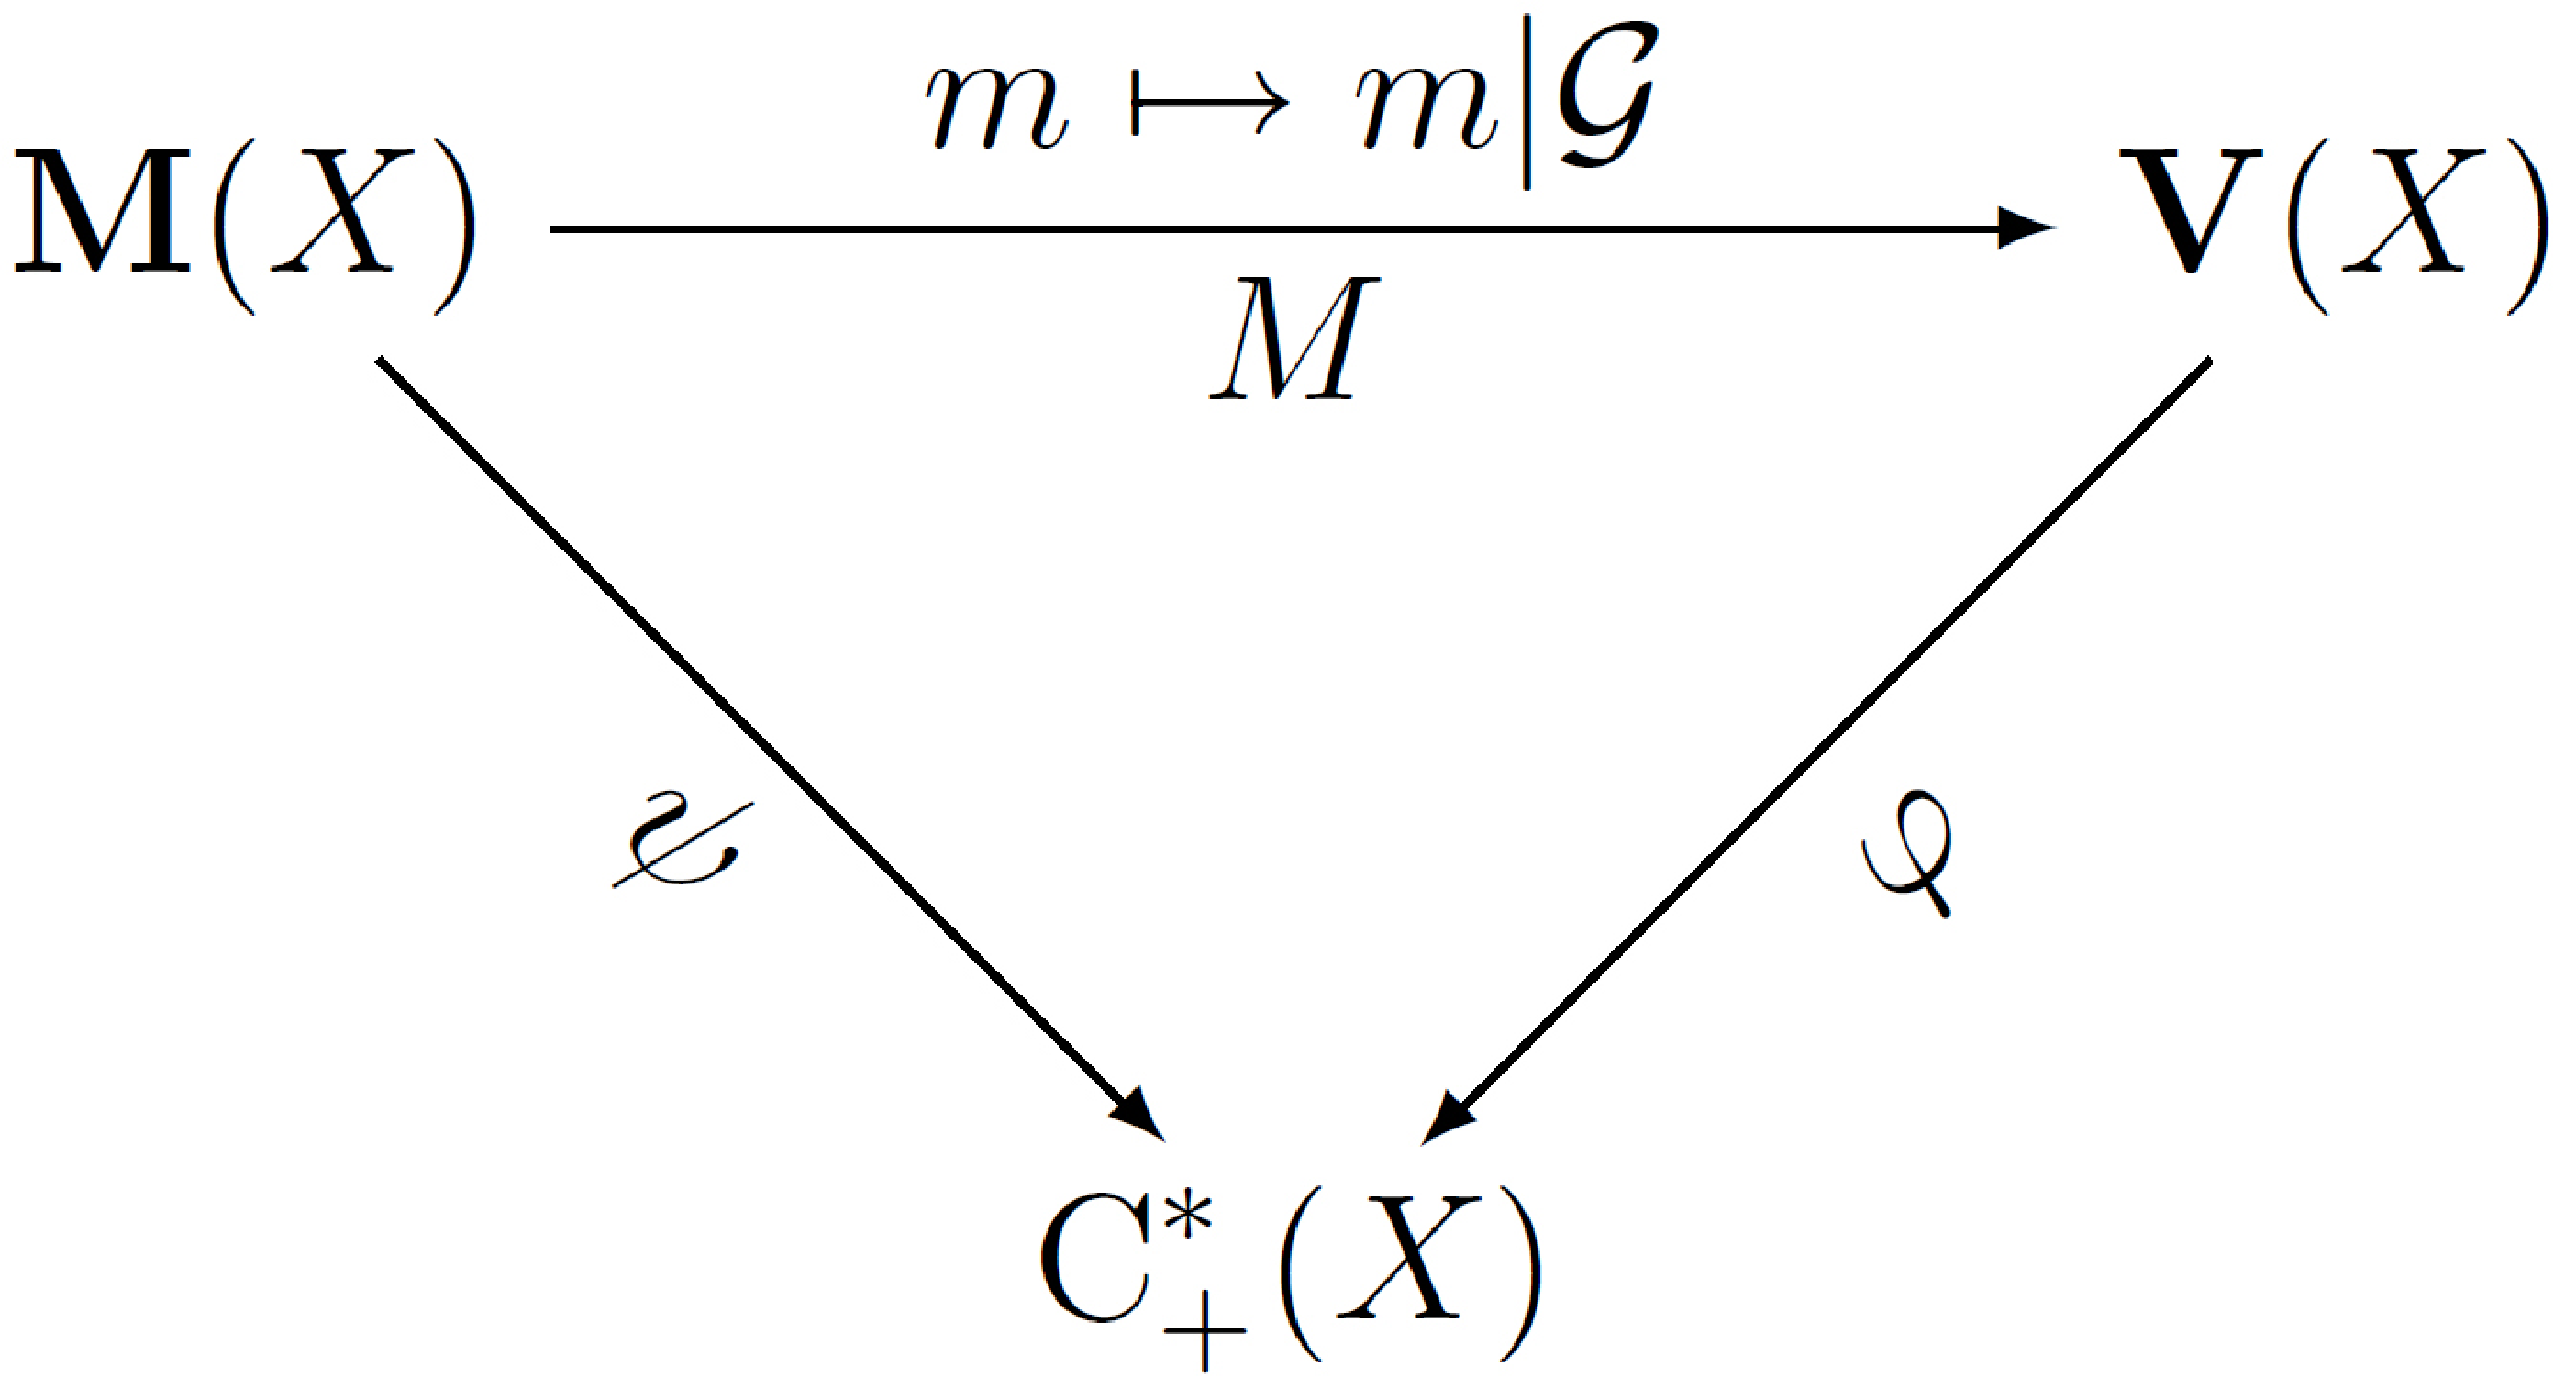
\includegraphics[height=3.2cm]{diagram.pdf}}
%\caption{}
\end{figure}

این نمودار جابجایی است،  به عبارت دیگر، 
$ \psi=\varphi\circ M $.  در حقیقت فرض کنید 
$ m $
یک اندازه بورل منتظم روی 
$ X $
باشد و
$ \mu=M(m)=m|_{\cG} $.  باید ثابت کنیم که 
$ \psi_{m}=\varphi_{\mu} $.  فرمول‌های مربوط به انتگرال‌ها در بخش
\ref{2}
و
\ref{3}
نشان می‌دهند که
$ \int{f}dm=\int{f}d\mu $،  که از آنجا،  برای هر
$ f\in \rC_{+}^{\uparrow}(X) $
نتیجه می‌شود که
$ \psi_{m}(f)=\varphi_{\mu}(f) $.   از آنجا که فضای برداری تولید شده بوسیله 
$ \rC_{+}^{\uparrow}(X) $
بطور یکنواخت در 
$ \rC(X) $
چگال است لذا نتیجه می‌گیریم که 
$. \psi_{m}=\varphi_{\mu} $


حال می‌توانیم مطالب را خلاصه کنیم:
\begin{theorem}\label{5.4} 
فرض کنید 
$ (X,\cO,\leq) $
یک فضای مرتب فشرده باشد.  
\begin{description}
\item[(i)]
هر ارزیابی پیوسته کراندار 
$ \mu $
تعریف شده روی گردایه 
$ \cG=\cO^{\uparrow} $
از مجموعه‌های بالایی باز،  می‌تواند به یک اندازه بورل منتظم 
$ \overline{\mu} $
روی 
$ X $
بطور یکتا،  گسترش یابد.
\item[(ii)]
نگاشت‌های 
$ \mu\mapsto \overline{\mu}:\mathrm{V}(\cG)\rightarrow \rM(X) $
و
$ \mu\mapsto \varphi_{\mu}: \mathrm{V}(X)\rightarrow \rC_{+}^{*}(X) $،  نسبت به ترتیب‌های تصادفی 
$ \prec $
مربوطه،  یکریختی‌هایی از مخروط‌ها، و یکریختی‌های ترتیبی هستند.   زیرمجموعه محدب 
$ \mathrm{V}_{\leq 1}(X) $
بروی 
$ \rC_{\leq 1}^{*}(X) $
و
$ \rM_{\leq 1}(X) $
 به ترتیب نگاشته می‌شود،  و 
$ \mathrm{V}_{ 1}(X) $
به ترتیب بروی 
$ \rC_{ 1}^{*}(X) $
و
$ \rM_{ 1}(X) $
 نگاشته می‌شود.
\item[(iii)]
متناظر با ترتیب تصادفی  
$ \prec $
و ضعیف‌ترین توپولوژیی که برای آن،  نگاشت‌های
\linebreak
$ \mu\mapsto \int{f}d\mu: \mathrm{V}(X)\rightarrow \bR$
برای هر 
$ f\in  \rC_{ +}^{\uparrow}(X) $
پیوسته هستند،  زیرمجموعه‌های 
$ \mathrm{V}_{\leq 1}(X) $
و
$ \mathrm{V}_{ 1}(X) $
فضاهای مرتب فشرده هستند. 
\item[(iv)]
فضای مرتب فشرده 
$ X $،  با نگاشته‌ شدن هر
$ x\in X $
به ارزیابی نقطه‌ای 
$ \delta_{x} $، توپولوژیکی و نشانده شده ترتیبی در 
$ \mathrm{V}_{ 1}(X)  $
است.
\item[(v)]
گردایه  مجموعه‌های بالایی باز فضاهای مرتب فشرده 
$ \mathrm{V}_{\leq 1}(X) $
و
$ \mathrm{V}_{ 1}(X)  $، با 
  \linebreak
  ضعیف‌ترین توپولوژیی که برای آن،  نگاشت‌های
  \  \  
$ \mu \mapsto \mu(U) $
به ازای همه مجموعه‌های بالایی باز
$ U\subseteq X $
نیمه‌پیوسته پایینی هستند،  منطبق می‌شوند.
\end{description}
\end{theorem}

\begin{proof}
$\mathrm{(i)}$
در لم 
\ref{5.3}
دیدیم که یک ارزیابی پیوسته کراندار 
$ \mu $
روی 
$ \cG $،  یک تابعی خطی مثبت یکتای 
$ \varphi_{\mu} $
تعریف می‌کند بطوری که برای هر 
$ f\in  \rC_{ +}^{\uparrow}(X) $
داشته باشیم
$ .\varphi_{\mu}(f)=\int{f}d\mu $
%%%%%%%%%%%%%%%%%%     end of page 236   %%%
  بنا به قضیه نمایش ریس و  
\ref{5.2}، اندازه بورل منتظم یکتای 
$ \overline{\mu} $ وجود دارد 
بطوری که برای هر 
$ f\in \rC(X) $
داریم
$ \varphi_{\mu}(f)=\int{f}d\overline{\mu} $.   بنابراین،  
$ \overline{\mu} $
اندازه بورل منتظم یکتایی است که برای هر 
$ f\in  \rC_{ +}^{\uparrow}(X) $،
$ \int{f}d\overline{\mu}=\int{f}d\mu $.    برای یک مجموعه بالایی باز 
$U$،  تابع مشخصه \linebreak
$ \chi_{U} $،  نیمه‌پیوسته پایینی است.   بنا به لم
\ref{1.1}،  
$ \chi_{U} $
سوپریمم نقطه‌وار خانواده جهت‌دار توابع
$ f_{i}\in \rC_{ +}^{\uparrow}(X)$
است.   بنابراین 
$$ \overline{\mu}(U)=\int{\chi_{U}}d\overline{\mu}=\sup_{i} \int{f_{i}}d\overline{\mu}=\sup_{i}\int{f_{i}}d\mu=\int{\chi_{U}}d\mu=\mu(U) $$
  (در اینجا از این واقعیت استفاده کرده‌ایم که 
$ f\mapsto \int{f}d\overline{\mu} $
و
$ f\mapsto \int{f}d\mu $
سوپریمم خانواده‌های جهت‌دار را حفظ می‌کنند(
\ref{2.1}
و
\ref{3.1}
را ببینید)).   این
$\mathrm{(i)}$
را ثابت می‌کند.


$\mathrm{(ii)}$
از آنجا که 
$ \psi=\varphi \circ M $،  وبنا به 
\ref{5.2}،   
$ \psi $
دوسویی است،  لذا نتیجه می‌گیریم که 
$ \varphi $
پوشا است.  از آنجا که 
$ \varphi $
بنا به
\ref{5.3}
یک نشاننده ترتیبی و لذا یک به یک است،  لذا نتیجه می‌گیریم که 
$\varphi  $،  دوسویی نیز هست و چون 
$ M=\psi\circ \varphi^{-1} $،  لذا $ M $ نیز دوسویی  است.


$\mathrm{(iii)}$
از گزاره
\ref{4.1}
و با استفاده از 
$ \mathrm{(ii)} $
نتیجه می‌شود.


$ \mathrm{(iv)} $
از
\ref{4.2}،   و
$ \mathrm{(v)} $
از لم
\ref{3.2}
  نتیجه می‌شود.
\end{proof}



قسمت‌های مختلف قضیه قبل،  قبلاً ثابت شده‌اند.   قسمت
$ \mathrm{(i)} $
مربوط به لاوسون
\cite{lawson}
است.   برای دامنه‌های فشرده لاوسون،   جانگ و تیکس\LTRfootnote{Jung and Tix}
\cite{Jung and Tix}
نشان داده‌اند که دامنه‌های توانی احتمالی 
$ \rV_{\leq1}(X) $
و
$ \rV_{1}(X)$، باز،  فشرده لاوسون هستند. این حالت خاصی از قسمت 
$ \mathrm{(iii)} $
قضیه قبل است.  همچنین  ام. آلوارز-مانیلا
\LTRfootnote{M.Alvarez-Manilla}
\cite{Alvarez2,Alvarez1}، پی برده است که ترتیب 
$ \prec $
برای ارزیابی‌ها، بیشتر با ترتیب تصادفی اندازه‌های احتمال،  که پیش از این توسط
 دی.ای. ادوارد در سال ۱۹۷۰ مطرح شده، ارتباط دارد 
\cite{D.A. Edwards}.  او نشان داده است که برای فضای مرتب فشرده 
$ X $،  
$ \rM_{\leq 1}(X) $
و
$ \rM_{1}(X) $،  فضاهای مرتب فشرده هستند.   قسمت
$ \mathrm{(v)}  $
از قضیه ایجاب می‌کند که برای یک فضای فشرده پایدار
$ X $،   دامنه های توانی احتمالی 
$ \rV_{\leq 1}(X) $
و
$ \rV_{ 1}(X) $
باز دوباره فشرده پایدار باشند.   این امر همچنین توسط آلوارز-مانیلا ثابت شده است
\cite{Alvarez2}.
%دستوراتی که برای تایپ تعاریف، قضایا، لم‌ها، مثال‌ها و ... به آنها نیاز دارید
%\begin{definition}
%\end{definition}
%\begin{theorem}
%\end{theorem}
%\begin{proposition}
%\end{proposition}
%\begin{example}
%\end{example}
%\begin{solution}
%\end{solution}
%\begin{remark}
%\end{remark}
%\begin{corollary}
%\end{corollary}


%%%%%%%%%%%%%%%%%    Referrences   %%%
%دستوراتی برای به حالت عادی در آمدن اندازه فونت‌ها و فاصله بین خطوط
\newpage
\normalsize
\small
%دستوری برای ظاهر شدن کلمه«مراجع» در فهرست مطالب
%\addcontentsline{toc}{section}{مراجع}
%ایجاد «مراجع»
\setLTRbibitems
\begin{thebibliography}{99}
\resetlatinfont
% چنانچه مرجع فارسی هم دارید باید یا از بسته Persian-bib استفاده کنید و یا راهنمای bidi را ملاحظه فرمایید. 

\bibitem{abramsky2}
S. Abramsky, A. Jung, {\em Domain theory}, in: S. Abramsky, D.M. Gabbay, T.S.E. Maibaum (Eds.), Handbook of
Logic in Computer Science, Vol. 3, Clarendon Press, Oxford, 1994, pp. 1–68.

\bibitem{aliprantis}
C.D. Aliprantis and O. Burkinshaw,   {\em Principles of Real Analysis}.  Academic Press.  1998,  xii+415 pp.

\bibitem{Alvarez1}
M. Alvarez-Manilla, {\em Measure theoretic results for continuous valuations on partially ordered
spaces}, Dissertation, Imperial College, London, 2000.

\bibitem{Alvarez2}
M. Alvarez-Manilla, {\em Extension of valuations on locally compact sober spaces}, Topology and its
Applications, 124, 2002 397-433.

\bibitem{Billingsley}
P. Billingsley, {\em Probability and Measure}, 2nd Edition, John Wiley \& Sons, 1986.

\bibitem{D.A. Edwards}
D.A. Edwards, {\em On the existence of probability measures with given marginals}, Annales de
l’Institut Fourier, Grenoble 28 1978, 53–78.

\bibitem{G. Gierz}
G. Gierz, K.H. Hofmann, K. Keimel, J.D. Lawson, M. Mislove, and D.S. Scott. {\em Continuous
Lattices and Domains}, Encyclopedia of Mathematics and its Applications 93, Cambridge
University Press, 2003, xxxvi+591pp.

\bibitem{Halmos}
P. Halmos, {\em Measure Theory}, D. Van-Nostrand Company, 1950.

\bibitem{Jones}
C. Jones,  {\em Probabilistic Non-Determinism}. PhD thesis, University of Edinburgh, Edinburgh,
1990. Also published as Technical Report No. CST-63-90.

\bibitem{Jung}
A. Jung,  {\em Cartesian Closed Categories of Domains}, volume 66 of CWI Tracts. Centrum voor
Wiskunde en Informatica, Amsterdam, 1989, 107 pp.

\bibitem{Kegelmann}
A. Jung, M. Kegelmann, and M.A. Moshier,  {\em Multi lingual sequent calculus and coherent spaces}.
Electronic Notes in Theoretical Computer Science, 6, 1997.

\bibitem{main}
K. Keimel, {\em The Probabilistic Powerdomain for Stably Compact Spaces via Compact Ordered Spaces}, Electronic Notes in Theoretical Computer Science 87, 2004 225–238.

\bibitem{Jung and Tix}
A. Jung and R. Tix,  {\em The troublesome probabilistic powerdomain}. Electronic Notes in
Theoretical Computer Science, 13, 1998.

\bibitem{Konig}
H. K¨onig,  {\em Measure and Integration}, Springer–Verlag, 1997, xxi+260 pp.

\bibitem{lawson}
J.D. Lawson, {\em Valuations on continuous lattices}. In: Math. Arbeitspapiere 27, Univ. Bremen,
1982, Ed. R.-E. Hoffmann, 204–225.

\bibitem{lawson 2}
J.D. Lawson, {\em Domains, Integration, and Positive Analysis}. Mathematical Structures in
Computer Science, 14, 2004, 815-832.

\bibitem{Nachbin}
L. Nachbin, {\em Topology and Order}. Van-Nostrand, Princeton, N.J., 1965.

\bibitem{rudin} 
W. Rudin,  {\em Real and Complex Analysis}.  Mc Graw-Hill Book Comp. 1966, xi+412 pp.

\bibitem{functional}
W. Rudin,  {\em Functional Analysis},  2nd Edition, Mc Graw-Hill Book Comp.  1991,  xv+424.

\bibitem{Tix} 
R. Tix,  {\em Stetige Bewertungen auf topologischen R¨aumen}. Diplomarbeit, Technische Universit¨at
Darmstadt, June 1995, 51 pp.

\end{thebibliography}

%\addcontentsline{toc}{section}{نمایه}
%دستوری برای ظاهر شدن کلمه «نمایه» در فهرست مطالب(البته در صورتی که از بسته‌ای که در ابتدا گفته شد استفاده %نکنید)
%ایجاد «نمایه»
\printindex

\end{document}